\documentclass[10pt,portuguese]{article}

\usepackage{fourier}

\usepackage[]{graphicx}
\usepackage[]{color}
\usepackage{xcolor}
\usepackage{alltt}
\usepackage{listings}
\usepackage[T1]{fontenc}
\usepackage[utf8]{inputenc}
\setlength{\parskip}{\smallskipamount}
\setlength{\parindent}{5ex}
\usepackage{indentfirst}
\usepackage{listings}
\usepackage{setspace}
\usepackage{hyperref}
\hypersetup{
    colorlinks=true,
    linkcolor=auburn,
    filecolor=magenta,      
    urlcolor=blue, urlsize=2em
}

% Set page margins
\usepackage[top=100pt,bottom=100pt,left=68pt,right=66pt]{geometry}

% Package used for placeholder text
\usepackage{lipsum}

% Prevents LaTeX from filling out a page to the bottom
\raggedbottom


\usepackage{fancyhdr}
\fancyhf{} 
\fancyfoot[C]{\thepage}
\renewcommand{\headrulewidth}{0pt} 
\pagestyle{fancy}

\usepackage{titlesec}
\titleformat{\chapter}
   {\normalfont\LARGE\bfseries}{\thechapter.}{1em}{}
\titlespacing{\chapter}{0pt}{50pt}{2\baselineskip}

\usepackage{float}
\floatstyle{plaintop}
\restylefloat{table}

\usepackage[tableposition=top]{caption}


\definecolor{light-gray}{gray}{0.95}

\renewcommand{\contentsname}{Índice}

\begin{document}


\begin{titlepage}
	\clearpage\thispagestyle{empty}
	\centering
	\vspace{2cm}

	
	{\Large  Sistemas Operativos \par}
	\vspace{0.5cm}
	{\small Professor: \\
	José Nuno Panelas Nunes Lau\par}
	\vspace{4cm}
	{ \textbf{Problema genérico de gestão de recursos:}} \\
	\vspace{0.5cm}
	{\Huge \textbf{Fumadores}} \\
	\vspace{1cm}
	\vspace{4cm}
	{\normalsize Carolina Araújo, 93248 \\ 
	             Hugo Paiva, 93195
	   \par}
	   	{\tiny
	Igual distribuição de trabalho \\entre os dois membros\par}
	\vspace{2cm}

    
\includegraphics[scale=0.20]{images/logo_ua.png}
    
    \vspace{2cm}
    
	{\normalsize DETI \\ 
		Universidade de Aveiro \par}
		
	{\normalsize 30-12-2019 \par}
	\vspace{2cm}
		
	
	\pagebreak

\end{titlepage}
\tableofcontents{}
\clearpage

\section{Introdução}
\par Este trabalho prático foi desenvolvido com o objetivo de compreender os mecanismos associados à execução de processos e \textit{threads}. 

\par Para empreender este propósito, foi pedido que se solucionasse um problema que envolve várias entidades que terão de colaborar entre si para um bom funcionamento do programa: os fumadores, os watchers e o agente. Dito isto, implementou-se um programa em \textit{C} que simula e soluciona o problema recorrendo a semáforos e a memória partilhada, de modo a sincronizar os vários processos independentes. 
\clearpage

\section{Contextualização}
\subsection{Processos e a utilização de múltiplas threads}
Uma thread é a unidade básica da utilização do CPU. Um processo que utilize múltiplas threads pode, portanto, realizar mais do que uma tarefa ao mesmo tempo. Isto traz benefícios como o \textbf{aumento na capacidade de resposta}, sendo que um programa pode continuar a correr mesmo que algumas threads estejam bloqueadas ou a realizar uma operação mais demorada. Ocorre também \textbf{partilha de recursos}, uma vez que os processos podem prestar os mesmos através da memória partilhada ou através do envio de mensagens. Há, de facto, um \textbf{menor gasto de memória}, uma vez que as múltiplas threads de um mesmo processo partilham entre si memória e dados, tornando-se mais eficiente usufruir das mesmas do que criar diferentes processos para realizar as mais variadas tarefas. Por fim, verifica-se também que em arquiteturas com \textbf{multiprocessadores}, as múltiplas threads podem estar a \textbf{correr em paralelo} nos diferentes processadores, o que, novamente, aumenta a eficiência de um processo.
\par O \textbf{cancelamento de threads} dá-se quando a tarefa realizada por uma thread é terminada antes de ser completada. A thread cancelada costuma ser referida como \textbf{target thread}, podendo terminar de duas maneiras: imediatamente através de uma outra thread (cancelamento assíncrono) ou verificando periodicamente se deve terminar (cancelamento síncrono). No entanto, isto pode acarretar problemas sendo que uma thread pode ser cancelada enquanto está num ponto vital, especialmente quando se trata do caso assíncrono, o que pode resultar numa recolha não total dos recursos do processo.
\subsection{Sincronização}
\par Considere-se agora um conjunto de processos. Caso esses partilhem uma variável que individualmente será, por eles, manipulada, pode acontecer o output acabar por não ser o esperado porque depende da ordem de manipulação dessa mesma variável. Isto é chamado de \textbf{condição de corrida}. Para combater algo do género, é necessário garantir que apenas um processo de cada vez pode estar a modificar esse tipo de variáveis partilhadas - ou seja, torna-se mandatório haver algum tipo de \textbf{sincronização}.
\par Cada processo tem um pedaço de código onde irá, possivelmente, alterar uma variável comum a todos os processos. Esta é chamada a \textbf{região crítica}. O mais importante, quando se trata de sincronização dos diferentes processos, é garantir que quando um deles entra na região crítica, mais nenhum pode entrar na região crítica que lhe compete. No entanto, se nenhum processo se encontra em execução numa destas regiões, caso um deles queira aceder, selecionar qual dos processos pode entrar é uma decisão que tem de ser tomada e não pode ser adiada indefinidamente. Terá, também, de haver um número limite de vezes que um dado processo tem acesso à região, sendo que outro pediu previamente acesso e ainda não lho foi garantido.
\par Os \textbf{semáforos}, uma solução hardware ao problema das regiões críticas, tornam-se vitais para sincronizar as tarefas realizadas pelas diferentes threads de um mesmo processo, permitindo também uma comunicação eficaz e fulcral entre as mesmas, para um bom funcionamento global. Um semáforo contém uma variável do tipo \textit{integer} que pode ser acedida de através de duas operações default: \textit{down()} e \textit{up()}, para além de quando se dá a sua inicialização. Estas duas operações têm como objetivo, respetivamente, entrar e sair na região crítica, bem como esperar por e entregar notificações. Modificações a essa variável através dessas funções são feitas de maneira indivisível. Isto é, quando uma das threads altera este valor, não poderá ser modificado simultaneamente por mais nenhuma. No caso de semáforos do tipo \textbf{mutex}, são \underline{semáforos binários} cujo valor pode apenas ser 0 ou 1, garantido sempre \textbf{exclusão mútua}. Existem também \underline{semáforos contadores} que podem ser utilizados para controlar o número de acessos a regiões críticas num dado processo.

\clearpage

\subsection{O problema dos Fumadores}

\par Este problema está relacionado com uma gestão de recursos envolvendo três fumadores com necessidades distintas para fumar, sendo que cada um deles possui apenas 1 recurso de fonte inesgotável. Para esta gestão existe uma entidade que disponibiliza/gera recursos e outras que necessitam/gastam recursos, sendo que estas necessidades envolvem vários recursos de tipos distintos. 
\par A dificuldade está em como fazer com que as entidades que necessitam dos recursos os usem nas alturas certas, sem que a entidade geradora de recursos faça a notificação direta às entidades gastadoras. Estas notificações vão ocorrer quando os pacotes que as entidades gastadoras necessitam estiverem completos e sem que tenham de fazer verificações desnecessárias para comprovar se já existem os recursos necessários.
\par \textbf{Para a resolução do problema existem algumas diretrizes:}
\begin{enumerate}
  \item O \textit{Agent} notifica o \textit{Watcher} responsável por cada ingrediente sempre que produz um ingrediente desse tipo.
  \item O \textit{Watcher} notifica o fumador sempre que ele pode fumar.
  \item Os \textit{Watchers} partilham informação entre si para comprovar que os 2 ingredientes estão disponíveis e poderem notificar o \textit{Smoker} correto.
  \item O \textit{Agent} apenas inicia um novo pacote quando o fumador já recolheu os ingredentes do pacote anterior.
  \item Após a produção de 5 pacotes, o \textit{Agent} termina a produção de recursos, notificando os \textit{Watchers} para que terminem. Estes por sua vez notificam os \textit{Smokers} para terminarem a sua execução.
\end{enumerate}
\par Na implementação da simulação deste problema foi utilizado o código-fonte disponibilizado pelo docente da disciplina onde já se encontravam definidos vários dados necessários à resolução.

\par Os recursos, tratados como ingredientes nesta implementação, que estão envolvidos neste processo são Tabaco, Fósforos e Papel. No ficheiro \textit{probConst.h} é possível encontrar estes ingredientes já definidos, bem como outros parâmetros gerais, úteis à implementação:

\begin{figure}[!h]
    \centering
    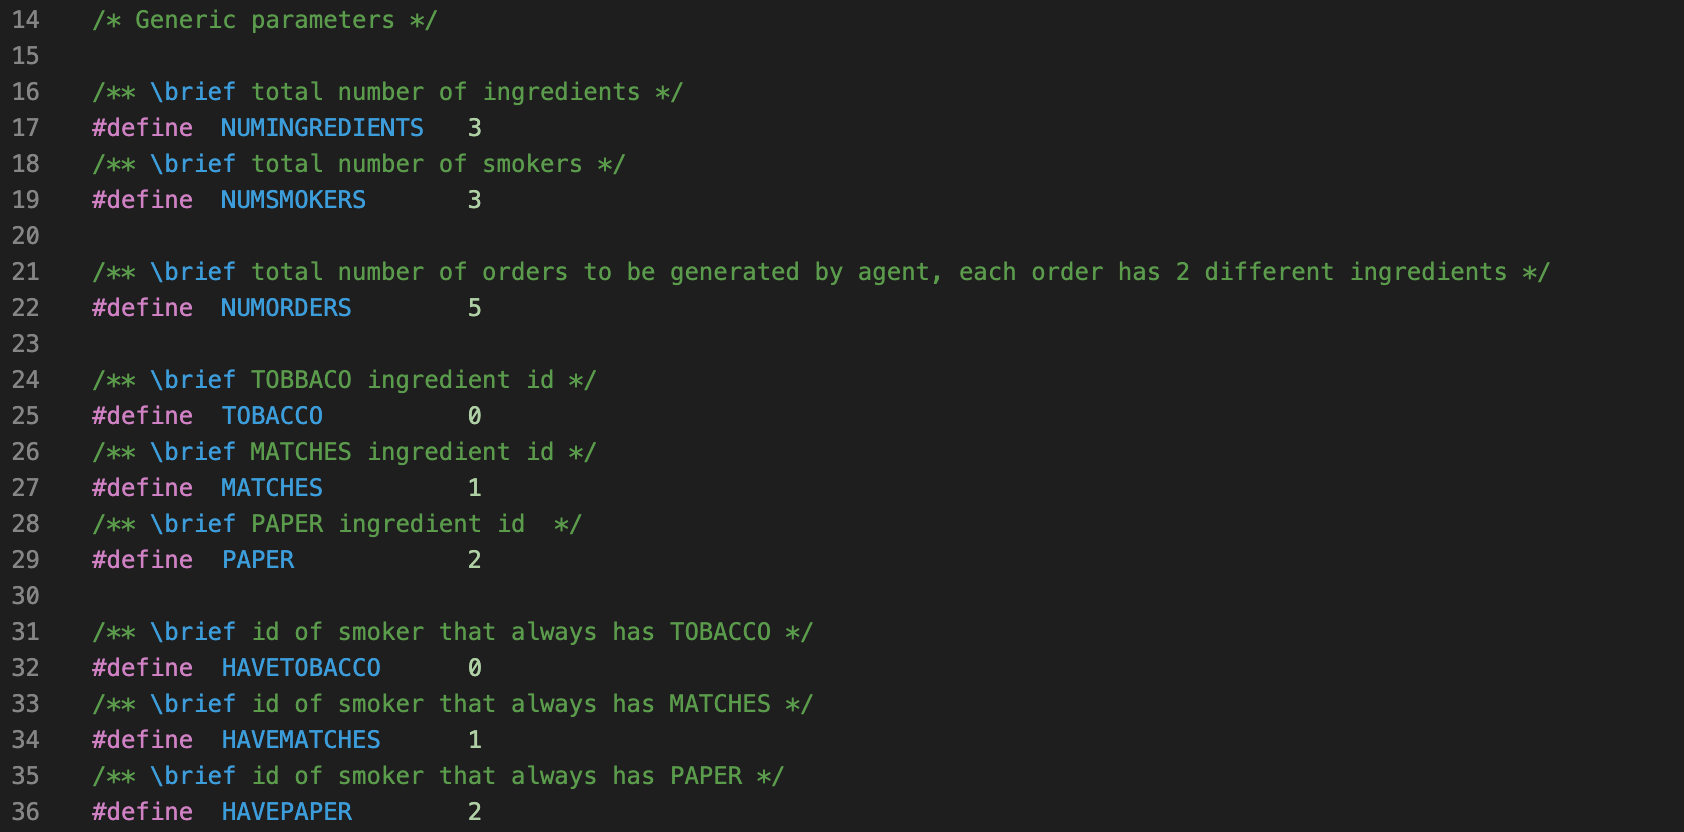
\includegraphics[scale=0.5]{images/Problem/generalparame.png}
    \caption{Parâmetros gerais definidos no ficheiro \textit{probConst.h}}
\end{figure}

\clearpage

\par Vão existir três entidades com as seguintes funções:
\begin{itemize}
  \item \textit{\textbf{Agent}} - Entidade que produz recursos em pacotes de 2 ingredientes distintos, ou seja, sempre que é produzido um pacote, apenas um fumador pode fumar. 
  \item \textit{\textbf{Watcher}} - Entidade responsável por verificar se, após a produção de um novo ingrediente de um pacote do \textit{Agente}, há algum fumador que pode fumar. Existe um watcher por cada ingrediente.
  \item \textit{\textbf{Smoker}} - Entidade que representa um fumador e que tem uma fonte inesgotável de um destes recursos, necessitando apenas dos outros 2.
\end{itemize}
\par Cada uma destas entidades têm vários estados associados à tarefa que estão atualmente a executar. Todos estes estados estão definidos, também, no ficheiro \textit{probConst.h}:

\begin{figure}[!h]
    \centering
    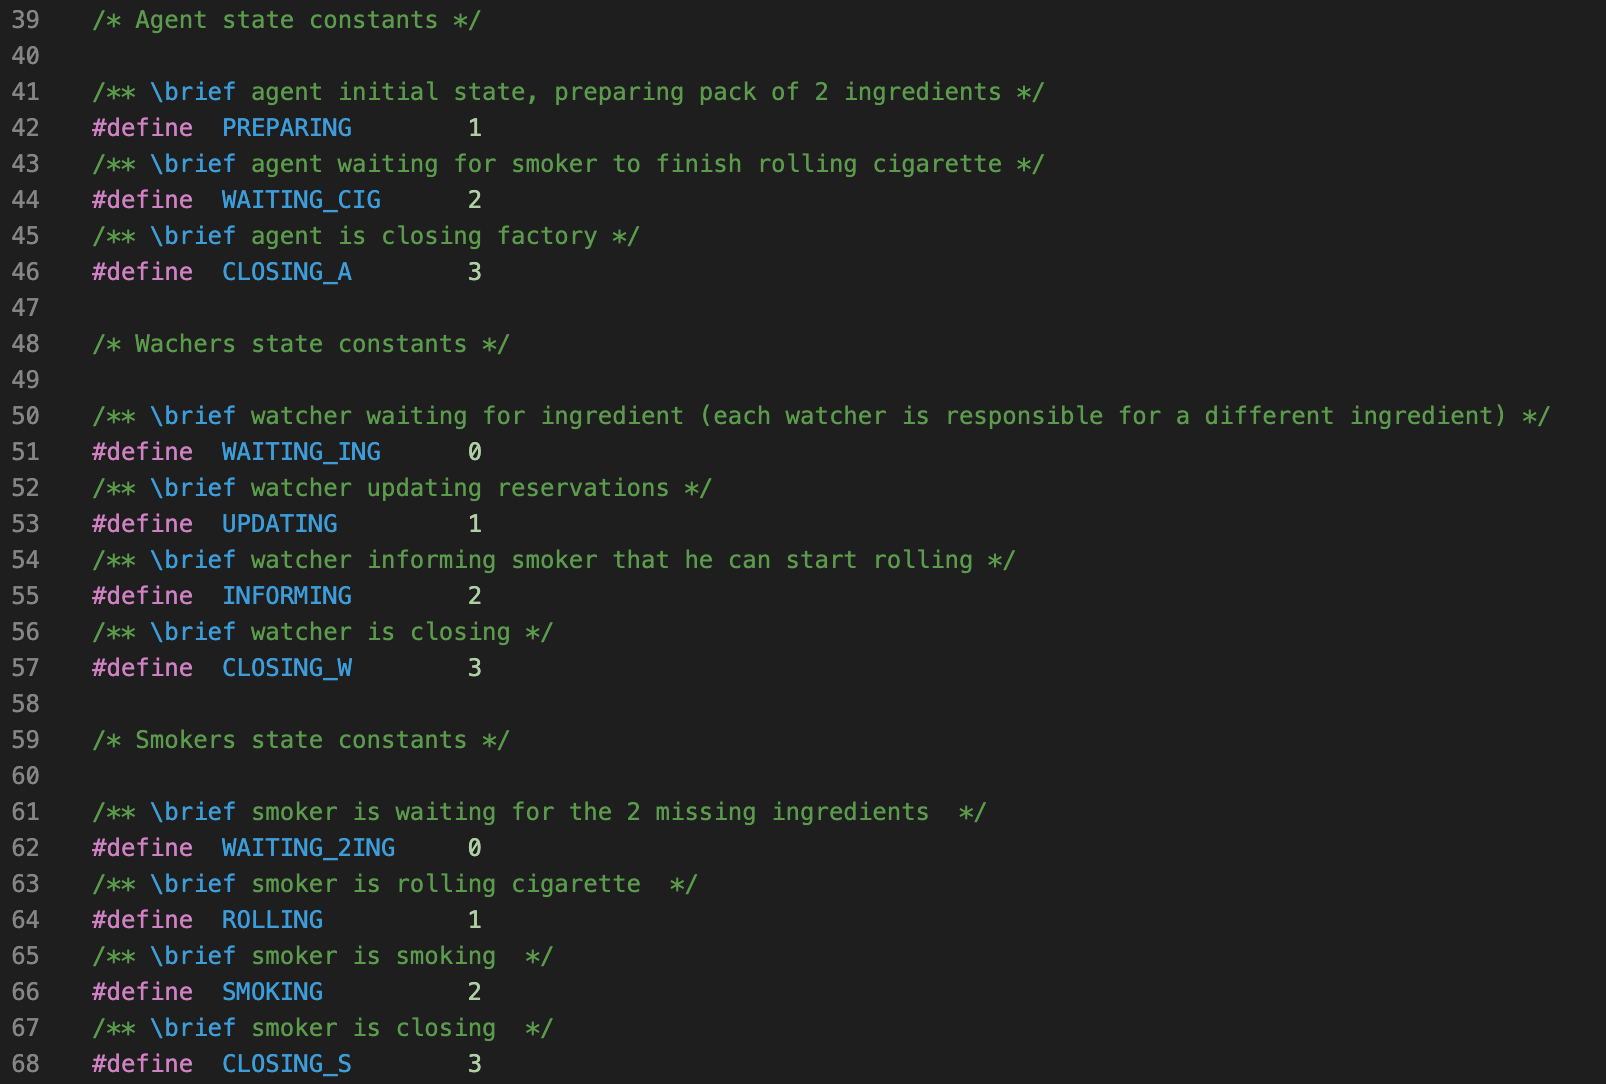
\includegraphics[width=\textwidth]{images/Problem/estados.png}
    \caption{Estados das várias entidades referentes ao problema, definidos no ficheiro \textit{probConst.h}}
\end{figure}
\clearpage
\par O conteúdo da memória partilhada é definido na estrutura \textit{FULL\_STAT} e no array dos 8 semáforos usados durante a implementação, no ficheiro \textit{sharedDataSync.h}:
\begin{figure}[!h]
    \centering
    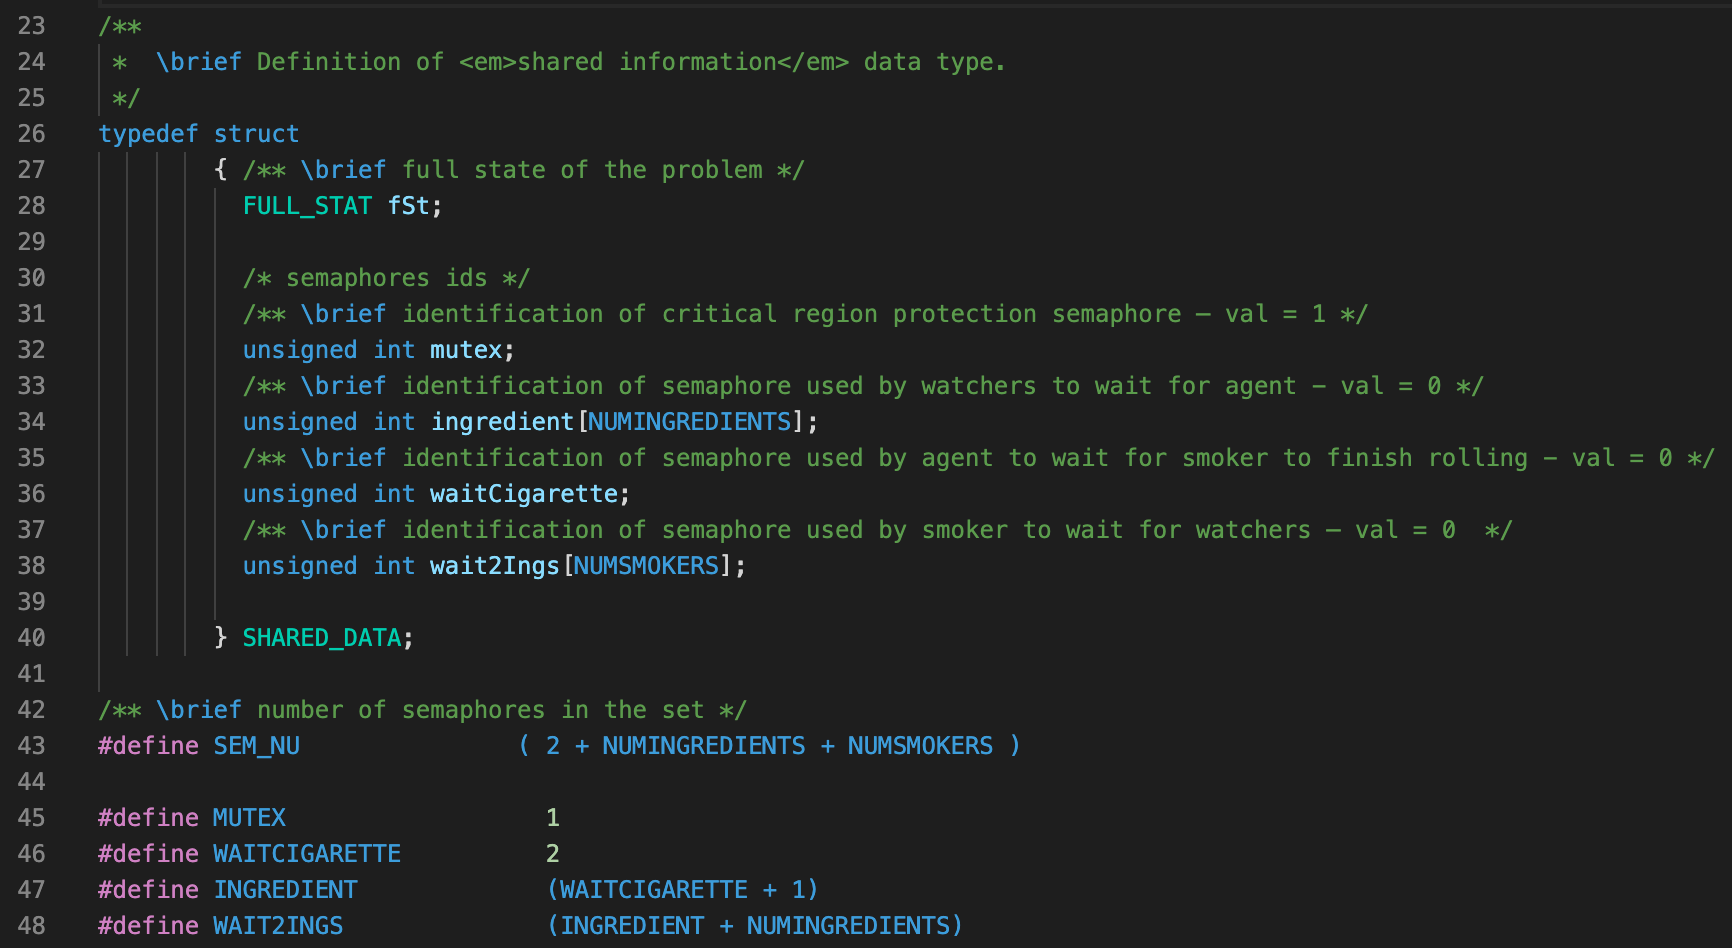
\includegraphics[width=\textwidth]{images/Problem/sharedmem.png}
    \caption{Definição dos tipos de dados e semáforos da memória partilhada no ficheiro \textit{sharedDataSync.h}}
\end{figure}
\clearpage
\par A definição das estruturas \textit{FULL\_STAT} e \textit{STAT}, usadas na memória partilhada, com os tipos de dados de todo o problema bem como o estado das entidades, encontram-se no ficheiro \textit{probDataStruct.h}:
\begin{figure}[!h]
    \centering
    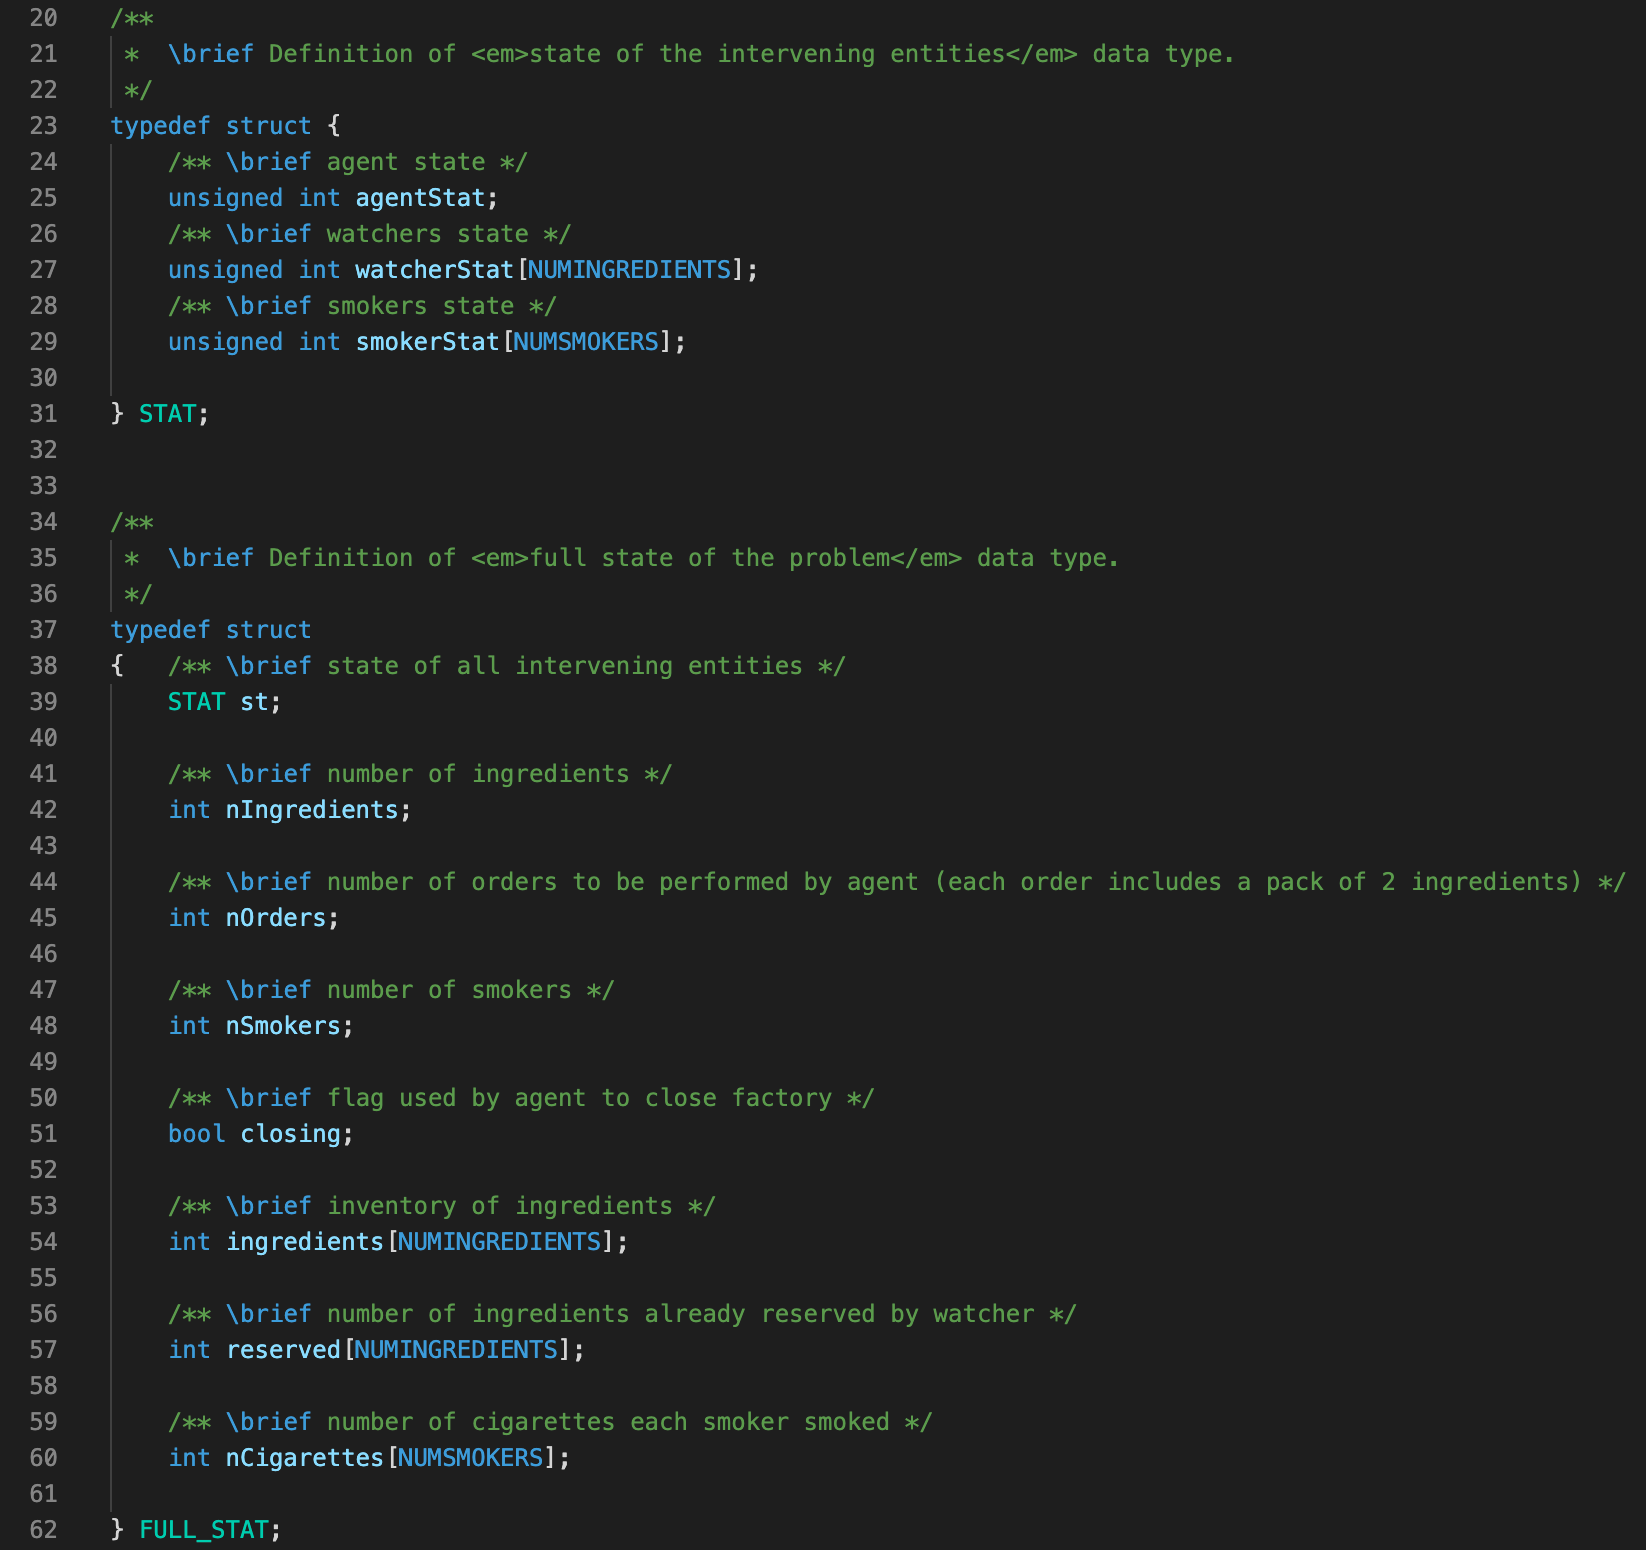
\includegraphics[width=\textwidth]{images/Problem/full_stat.png}
    \caption{Definição das estruturas \textit{FULL\_STAT} e \textit{STAT} no ficheiro \textit{probDataStruct.h}}
\end{figure}

\clearpage

\section{Implementação}

\par Recorrendo a semáforos e a memória partilhada, de modo a sincronizar os vários processos independentes, foi implementada uma resolução do problema a partir do código-fonte do professor. A explicação da implementação irá, portanto, inserir-se no código feito pelos alunos, nos locais e ficheiros definidos pelo docente da disciplina. 

\par A utilização dos semáforos ao longo da solução serviu principalmente para controlar o acesso à memória partilhada, evitando assim potenciais colisões que as 3 entidades poderiam vir a ter durante a sua execução. As notificações trocadas entre as entidades foram também implementadas usando semáforos, permitindo assim a contínua execução do programa. Para uma melhor interpretação deste funcionamento, foi feita uma tabela que associa cada semáforo à sua função durante a resolução:\\
\begin{figure}[!h]
    \centering
    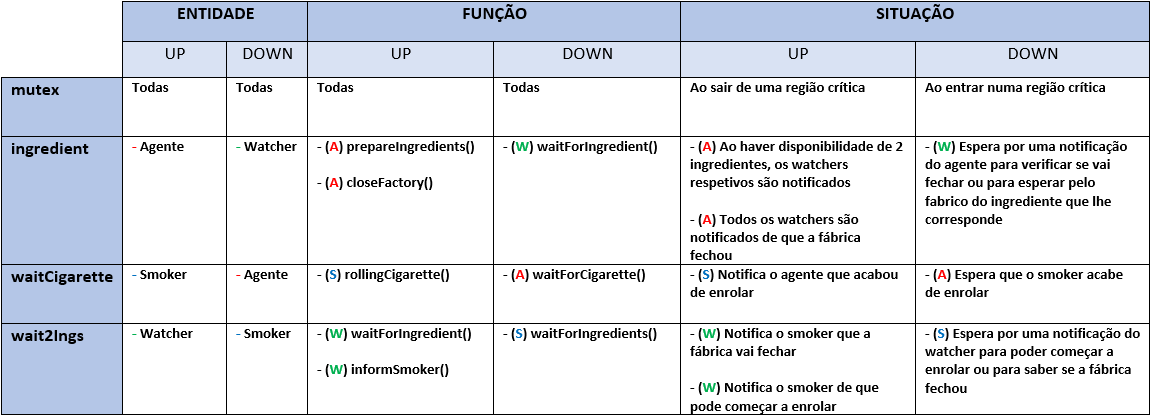
\includegraphics[width=\textwidth]{images/implementation/table.png}
    \caption{Tabela dos semáforos existentes e a sua utilização}
\end{figure}

\clearpage

\subsection{\textit{Agent}}

\par Começando por implementar a solução da entidade \textit{Agent}, foi necessário alterar o ficheiro \textit{semSharedMemAgent.c} nos locais assinalados. As funções \textit{prepareIngredients()}, \textit{waitForCigarette()} e \textit{closeFactory()} foram modificadas da maneira que se segue.

\subsubsection{\textit{prepareIngredients()}}

\par Nesta função o Agente prepara 2 ingredientes. Para isso, após entrar na região crítica com o uso da função \textit{semDown()}, é atualizado o seu estado para \textit{PREPARING}, escolhendo-se posteriormente, e de forma aleatória, os 2 ingredientes a fazerem parte do novo pacote. Após esta escolha, o inventário é atualizado com as novas existências, guardando-se estas novas alterações na memória partilhada. Já fora da região crítica, ambos os \textit{Watchers} referentes aos ingredientes gerados são notificados que os estes se encontram então disponíveis com o desbloqueio de dois semáforos pertencentes a cada ingrediente, através da função \textit{semUp()}.

\begin{figure}[!h]
    \centering
    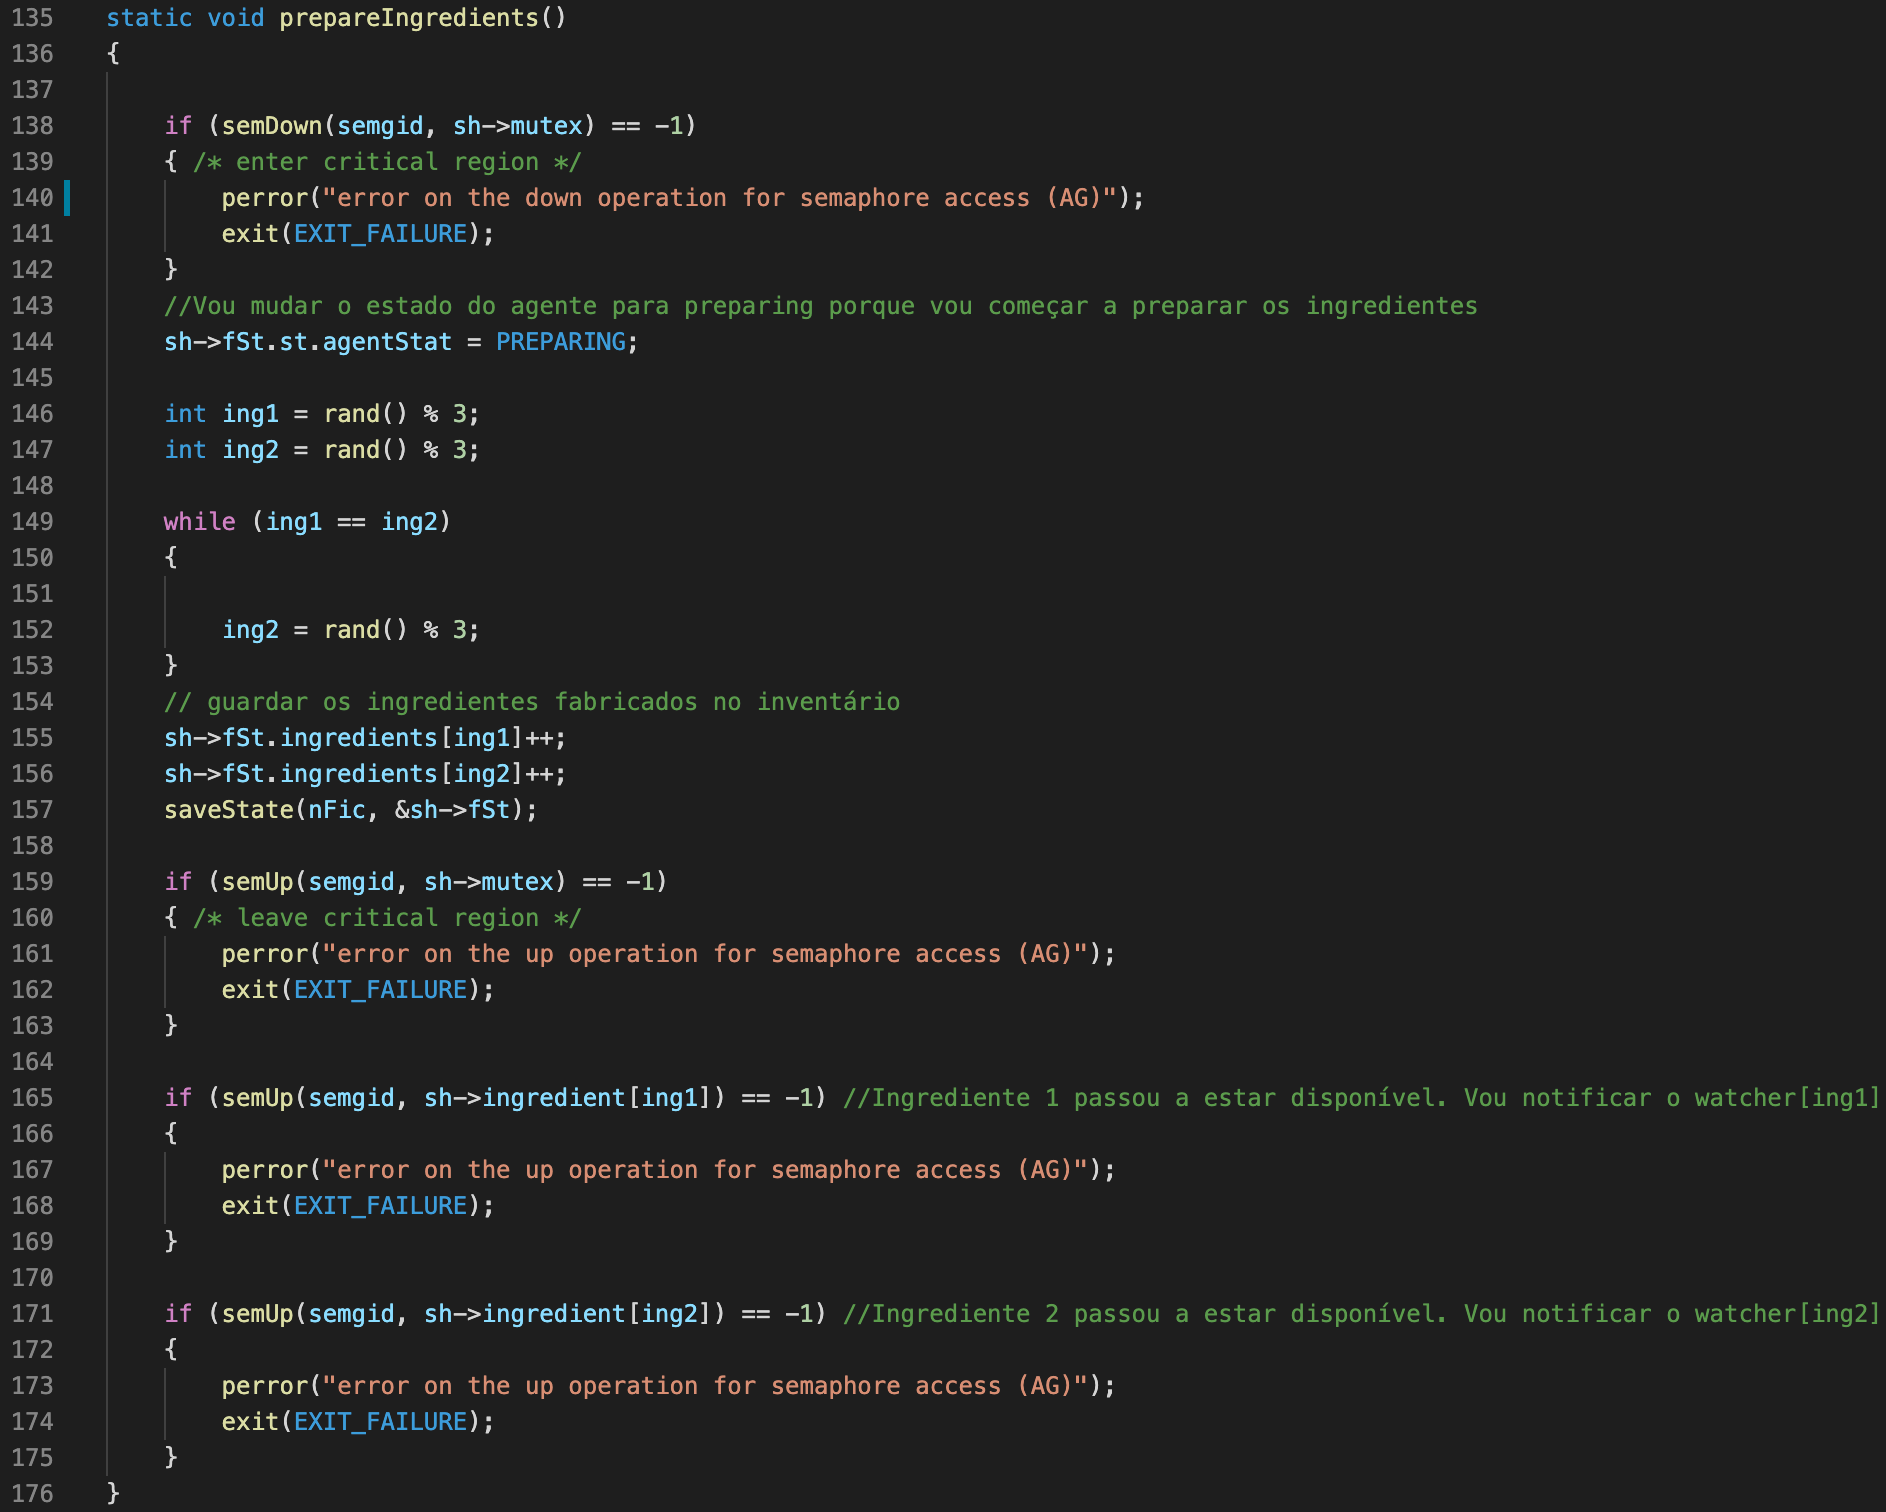
\includegraphics[width=\textwidth]{images/implementation/prepareings.png}
    \caption{Função \textit{prepareIngredients()}}
\end{figure}

\subsubsection{\textit{waitForCigarette()}}

\par Ao executar \textit{waitForCigarette()}, o Agente vai esperar que o Fumador acabe de enrolar o cigarro. Isto é alcançado entrando na região crítica, de modo a que o Agente altere o seu estado para \textit{WAITING\_CIG}, guardando-o depois na memória partilhada. Fora da região crítica, é feito um \textit{semDown()} para bloquear o semáforo \textit{waitCigarette}, o qual só é liberto quando o Fumador acabar de enrolar.

\begin{figure}[!h]
    \centering
    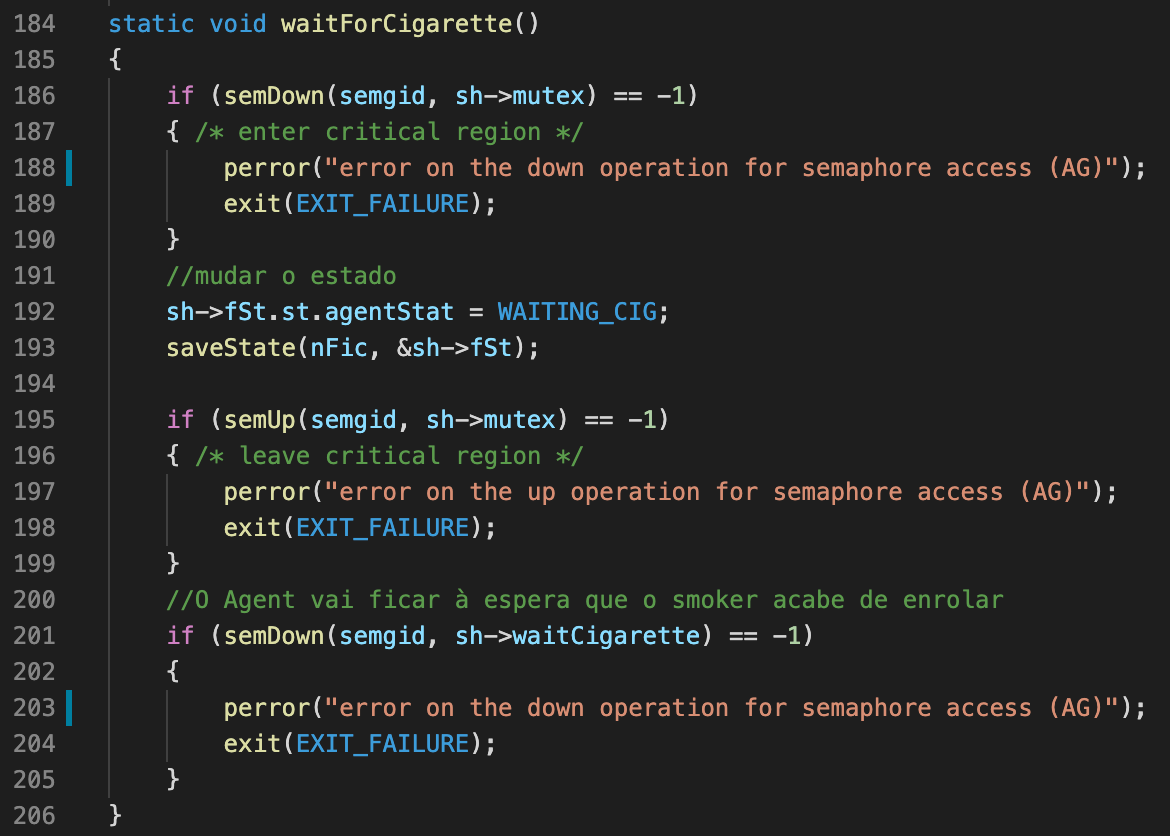
\includegraphics[width=\textwidth]{images/implementation/waitcig.png}
    \caption{Função \textit{waitForCigarette()}}
\end{figure}

\clearpage

\subsubsection{\textit{closeFactory()}}

\par Na função \textit{closeFactory()} o Agente vai terminar o fabrico de ingredientes, fechando a fábrica. Assim, dentro da região crítica, este atualiza o seu estado para \textit{CLOSING\_A} e altera a flag \textit{closing} para \textit{true} guardando estas alterações em memória partilhada. Fora da região crítica, são notificados os 3 \textit{Watchers} desbloqueando os semáforos referentes a cada ingrediente. Desta forma, todos os \textit{Watchers} vão entrar em funcionamento e verificar que a fábrica está a fechar.

\begin{figure}[!h]
    \centering
    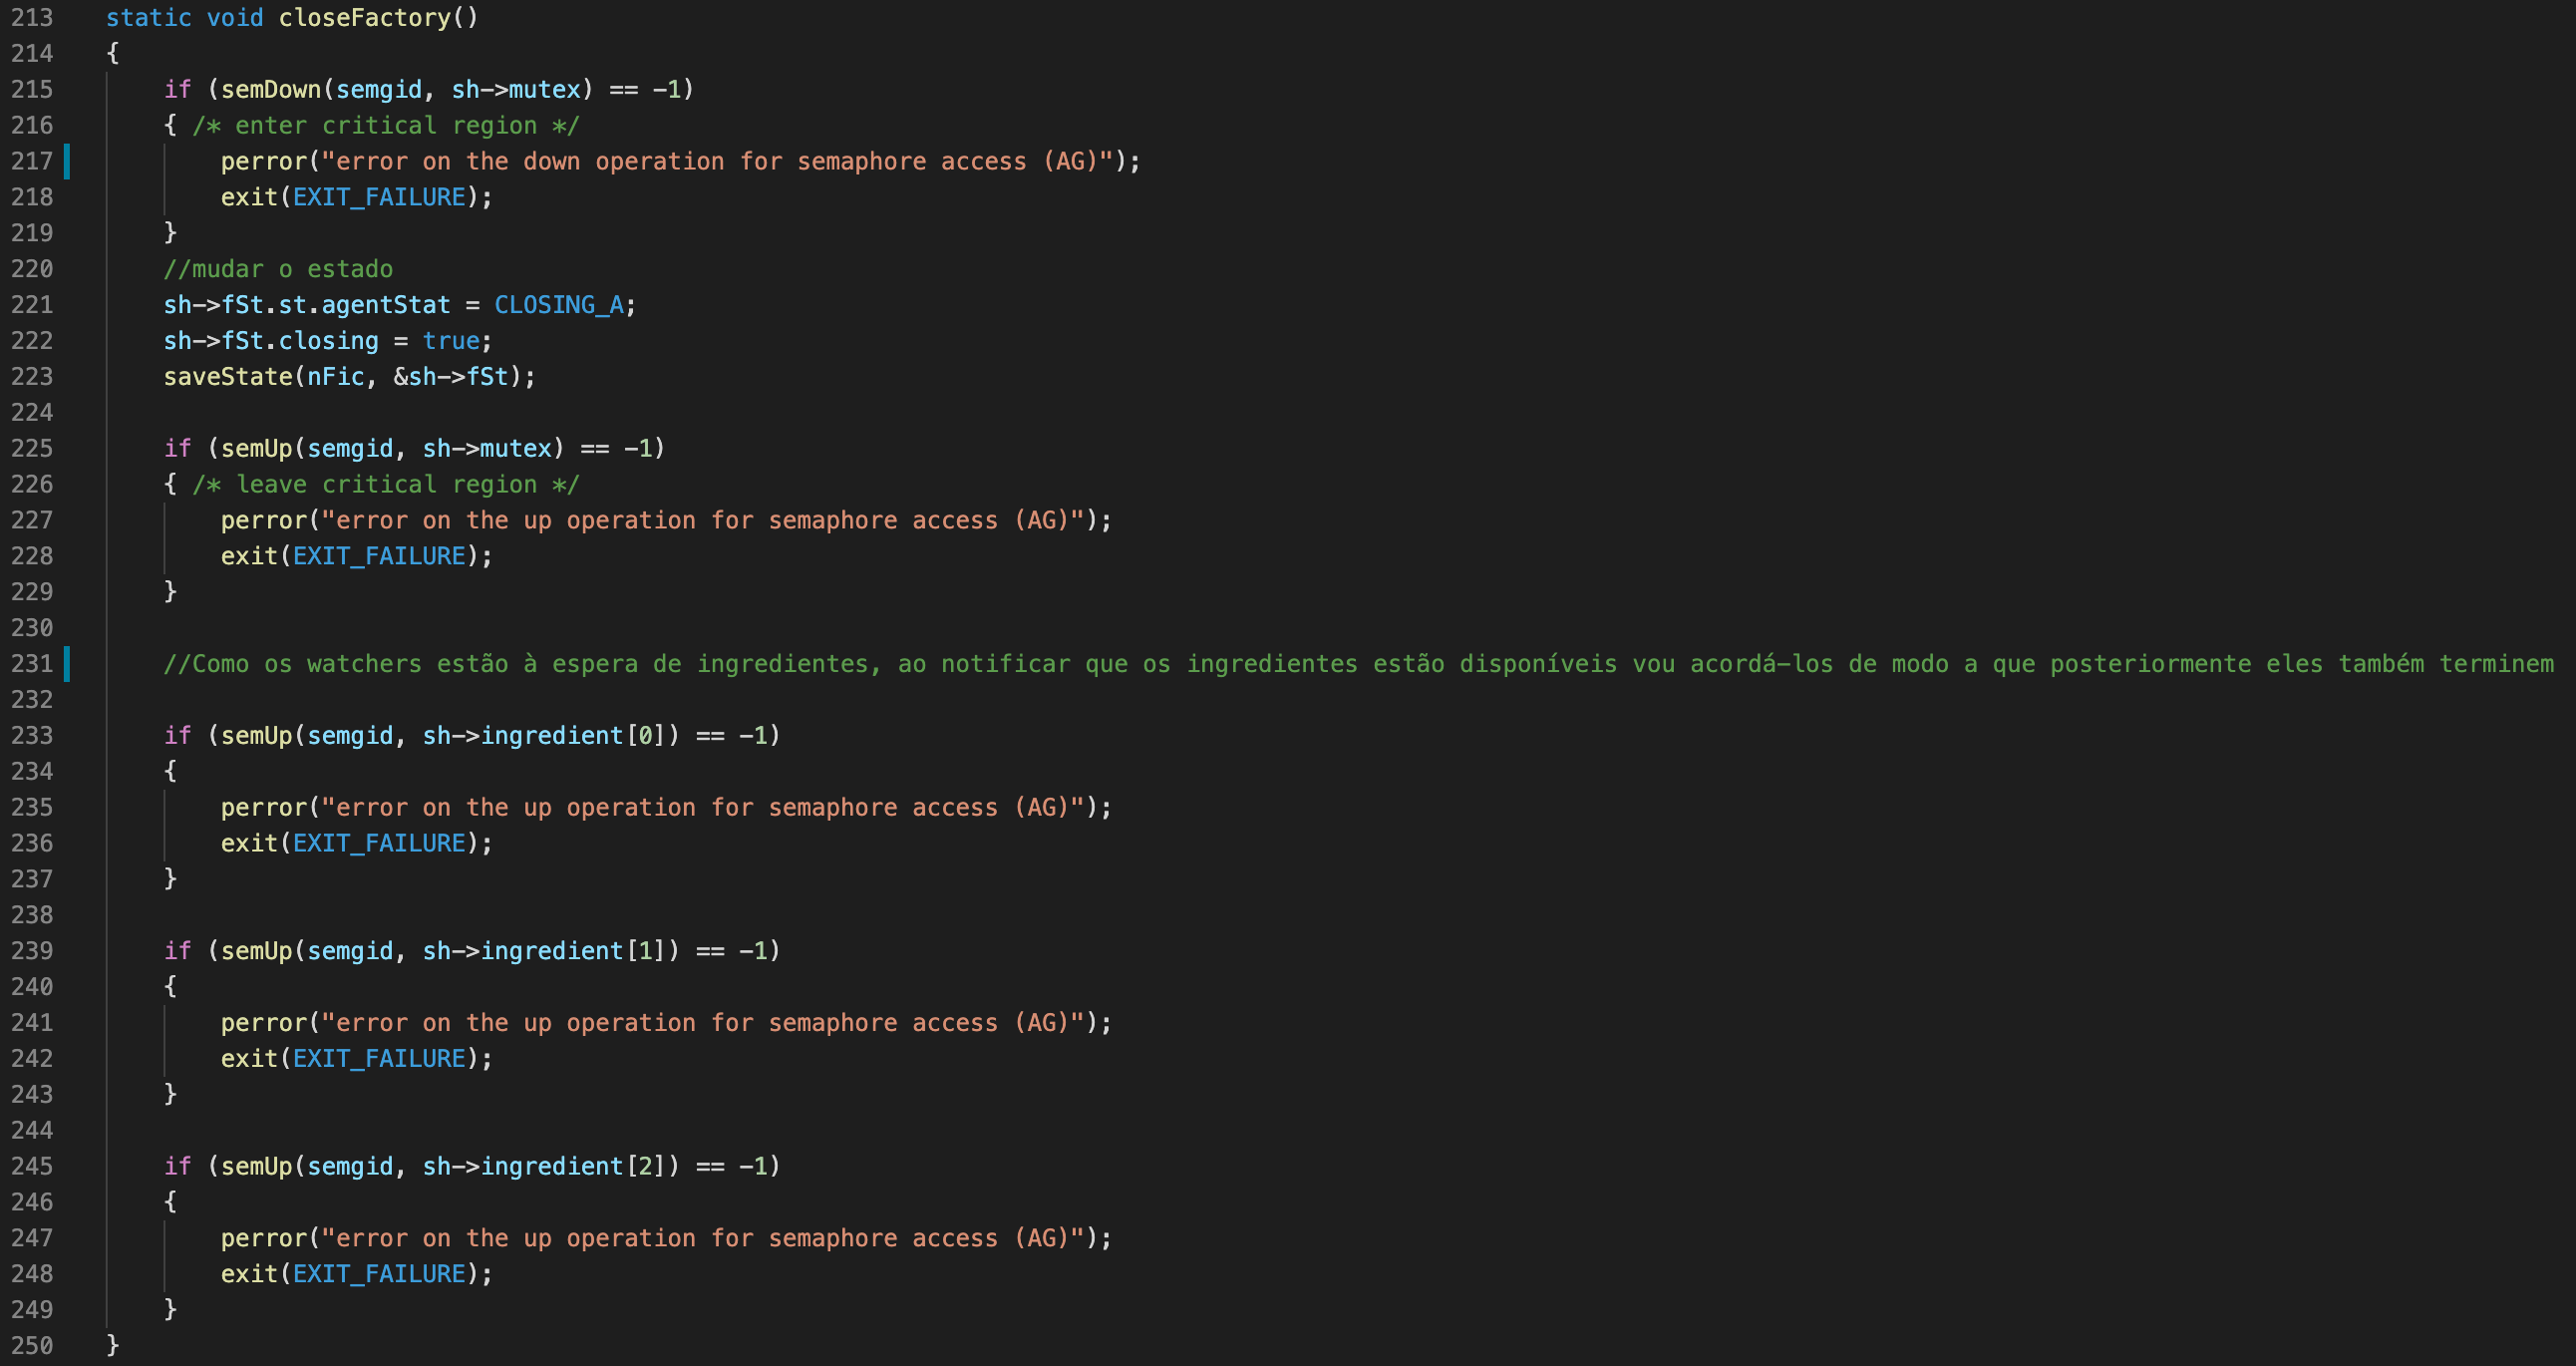
\includegraphics[width=\textwidth]{images/implementation/closefact.png}
    \caption{Função \textit{closeFactory()}}
\end{figure}

\subsection{\textit{Watcher}}
\par Ao implementar a solução da entidade \textit{Watcher} foi necessário alterar o ficheiro \textit{semSharedMemWatcher.c} nos locais assinalados. As funções \textit{waitForIngredient()}, \textit{updateReservations()} e \textit{informSmoker()} foram modificadas da maneira que se segue.

\subsubsection{\textit{waitForIngredient()}}

\par Nesta função o \textit{Watcher} espera que o seu ingrediente esteja pronto. Para isso, após entrar na região crítica, é atualizado o seu estado para \textit{WAITING\_ING}, guardando-o na memória partilhada. Já fora da região crítica, é bloqueado o semáforo referente ao ingrediente desta entidade, ficando esta à espera da disponibilidade desse ingrediente. Quando este semáforo voltar a estar desbloqueado, volta-se a entrar na região crítica, verificando-se se a flag \textit{closing} está a \textit{true}. Nesse caso, é atualizado o estado do \textit{Watcher} para \textit{CLOSING\_W}, guardando-se na memória partilhada e mudando o \textit{return} para \textit{false}, notificando, ainda, antes de sair da região crítica, o Fumador com o mesmo \textit{id} que o \textit{Watcher} em questão, para este também verificar se a fábrica está a fechar. Em caso contrário, não é feito nada.

\begin{figure}[!h]
    \centering
    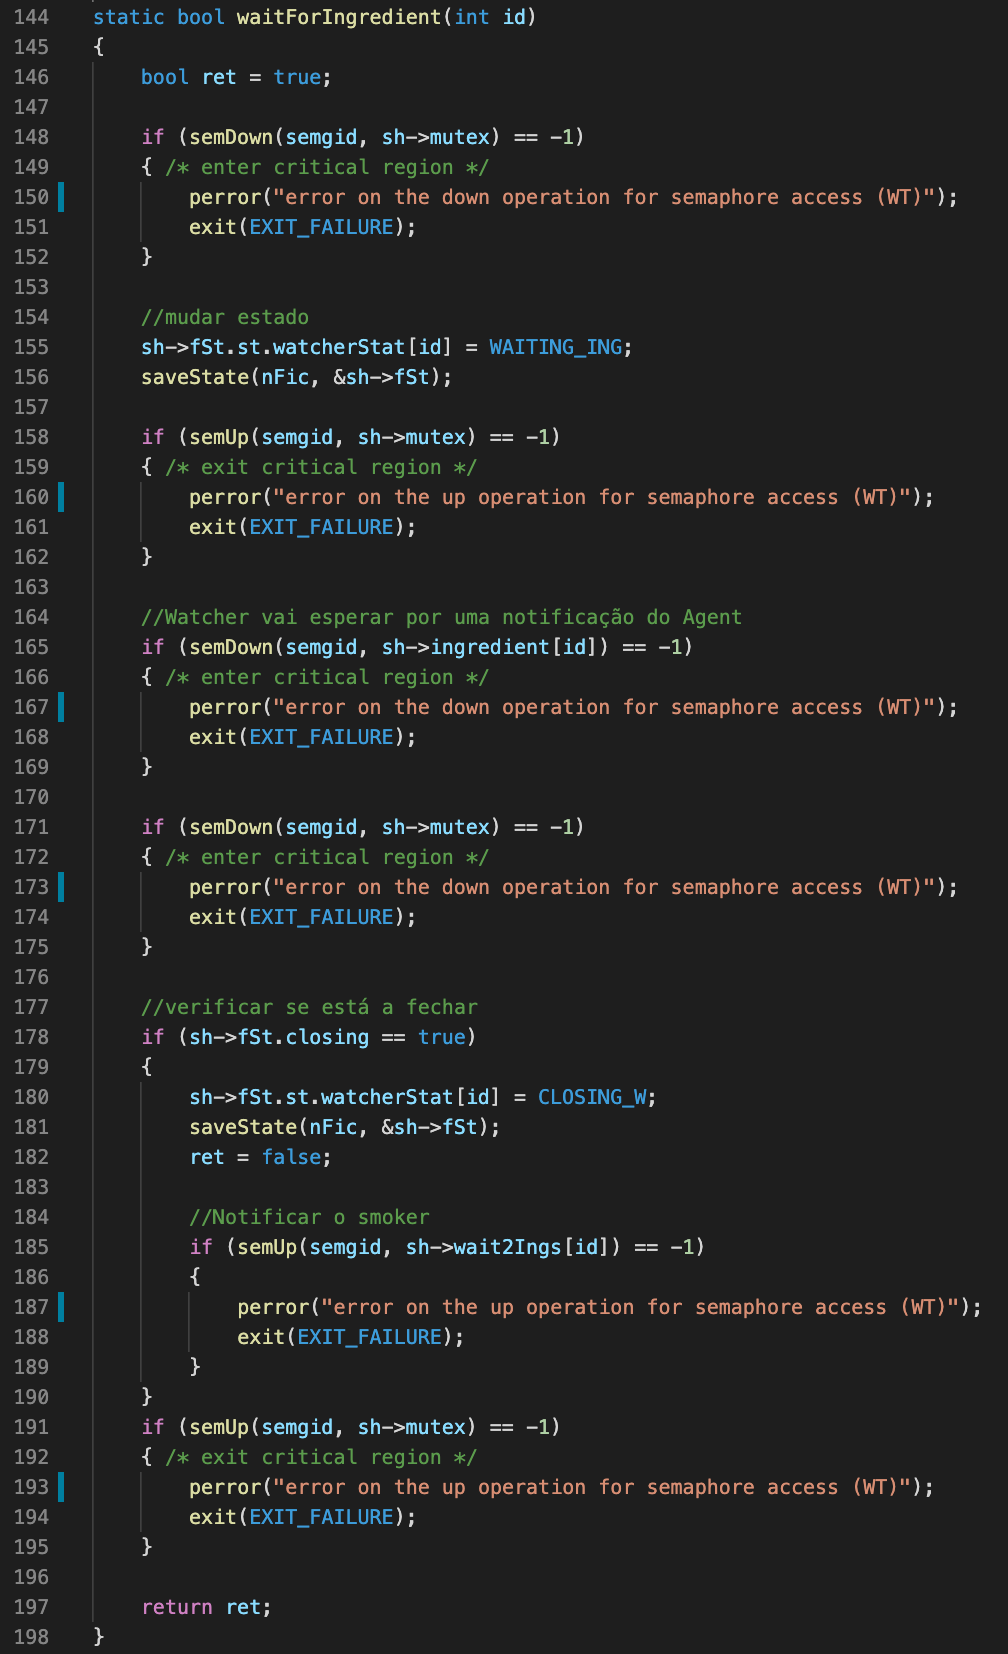
\includegraphics[scale=0.7]{images/implementation/waitforing.png}
    \caption{Função \textit{waitForIngredient()}}
\end{figure}

\clearpage

\subsubsection{\textit{updateReservations()}}

\par Ao executar \textit{updateReservations()} o \textit{Watcher} atualiza as reservas na memória partilha e verifica se algum Fumador pode fumar. Isto é alcançado entrando na região crítica, de modo a que o \textit{Watcher} altere o seu estado para \textit{UPDATING} e incremente 1 à posição correspondente ao seu ingrediente no \textit{array} dos ingredientes reservados, guardando estes dados na memória partilhada. Ainda dentro da região crítica, é verificado se algum Fumador pode fazer um cigarro. Assim, é analisado o \textit{array} de ingredientes reservados e, caso haja dois ingredientes com uma ou mais reservas, a função passa a retornar o \textit{id} do Fumador que não possui estes ingredientes.

\begin{figure}[!h]
    \centering
    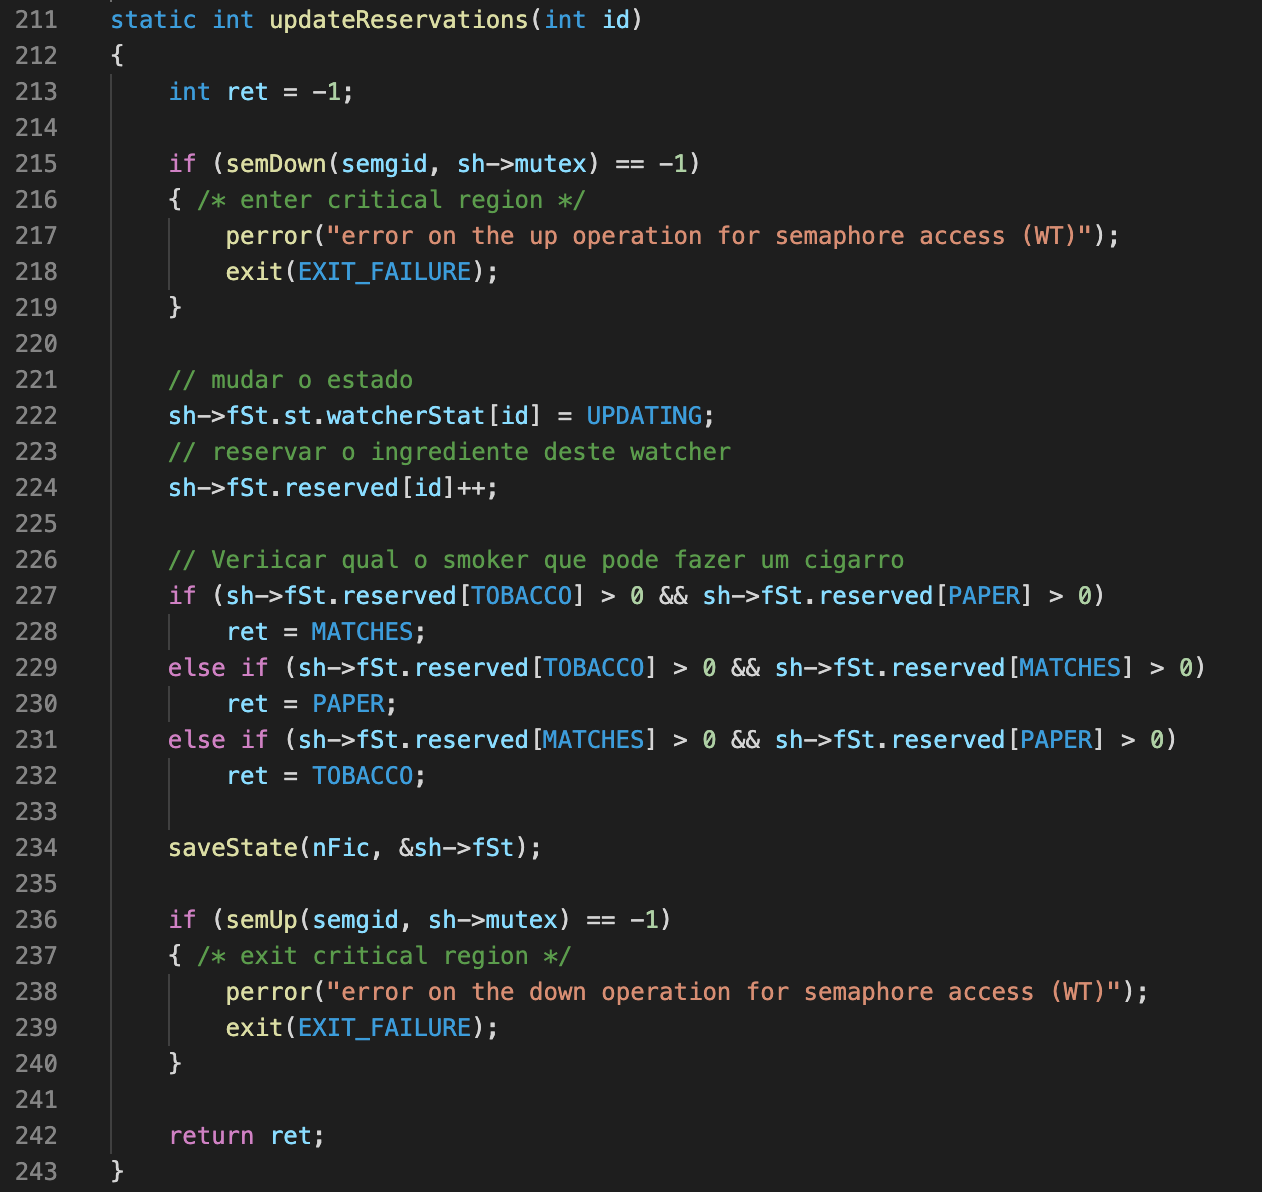
\includegraphics[width=\textwidth]{images/implementation/updateres.png}
    \caption{Função \textit{updateReservations(}}
\end{figure}

\clearpage

\subsubsection{\textit{informSmoker()}}

\par Na função \textit{informSmoker()} o \textit{Watcher} vai informar o Fumador que pode usar os ingredientes disponíveis para enrolar um cigarro. Assim, dentro da região crítica, é atualizado o seu estado para \textit{INFORMING} e retirada uma unidade aos ingredientes prestes a ser utilizados pelo Fumador do \textit{array} dos ingredientes reservados, guardando estas alterações em memória partilhada. Fora da região crítica, é notificado o Fumador que pode enrolar um cigarro através da variável \textit{smokerReady} que foi retornada na última função analisada, aliada ao desbloqueio do semáforo \textit{wait2Ings} referente ao Fumador em questão.

\begin{figure}[!h]
    \centering
    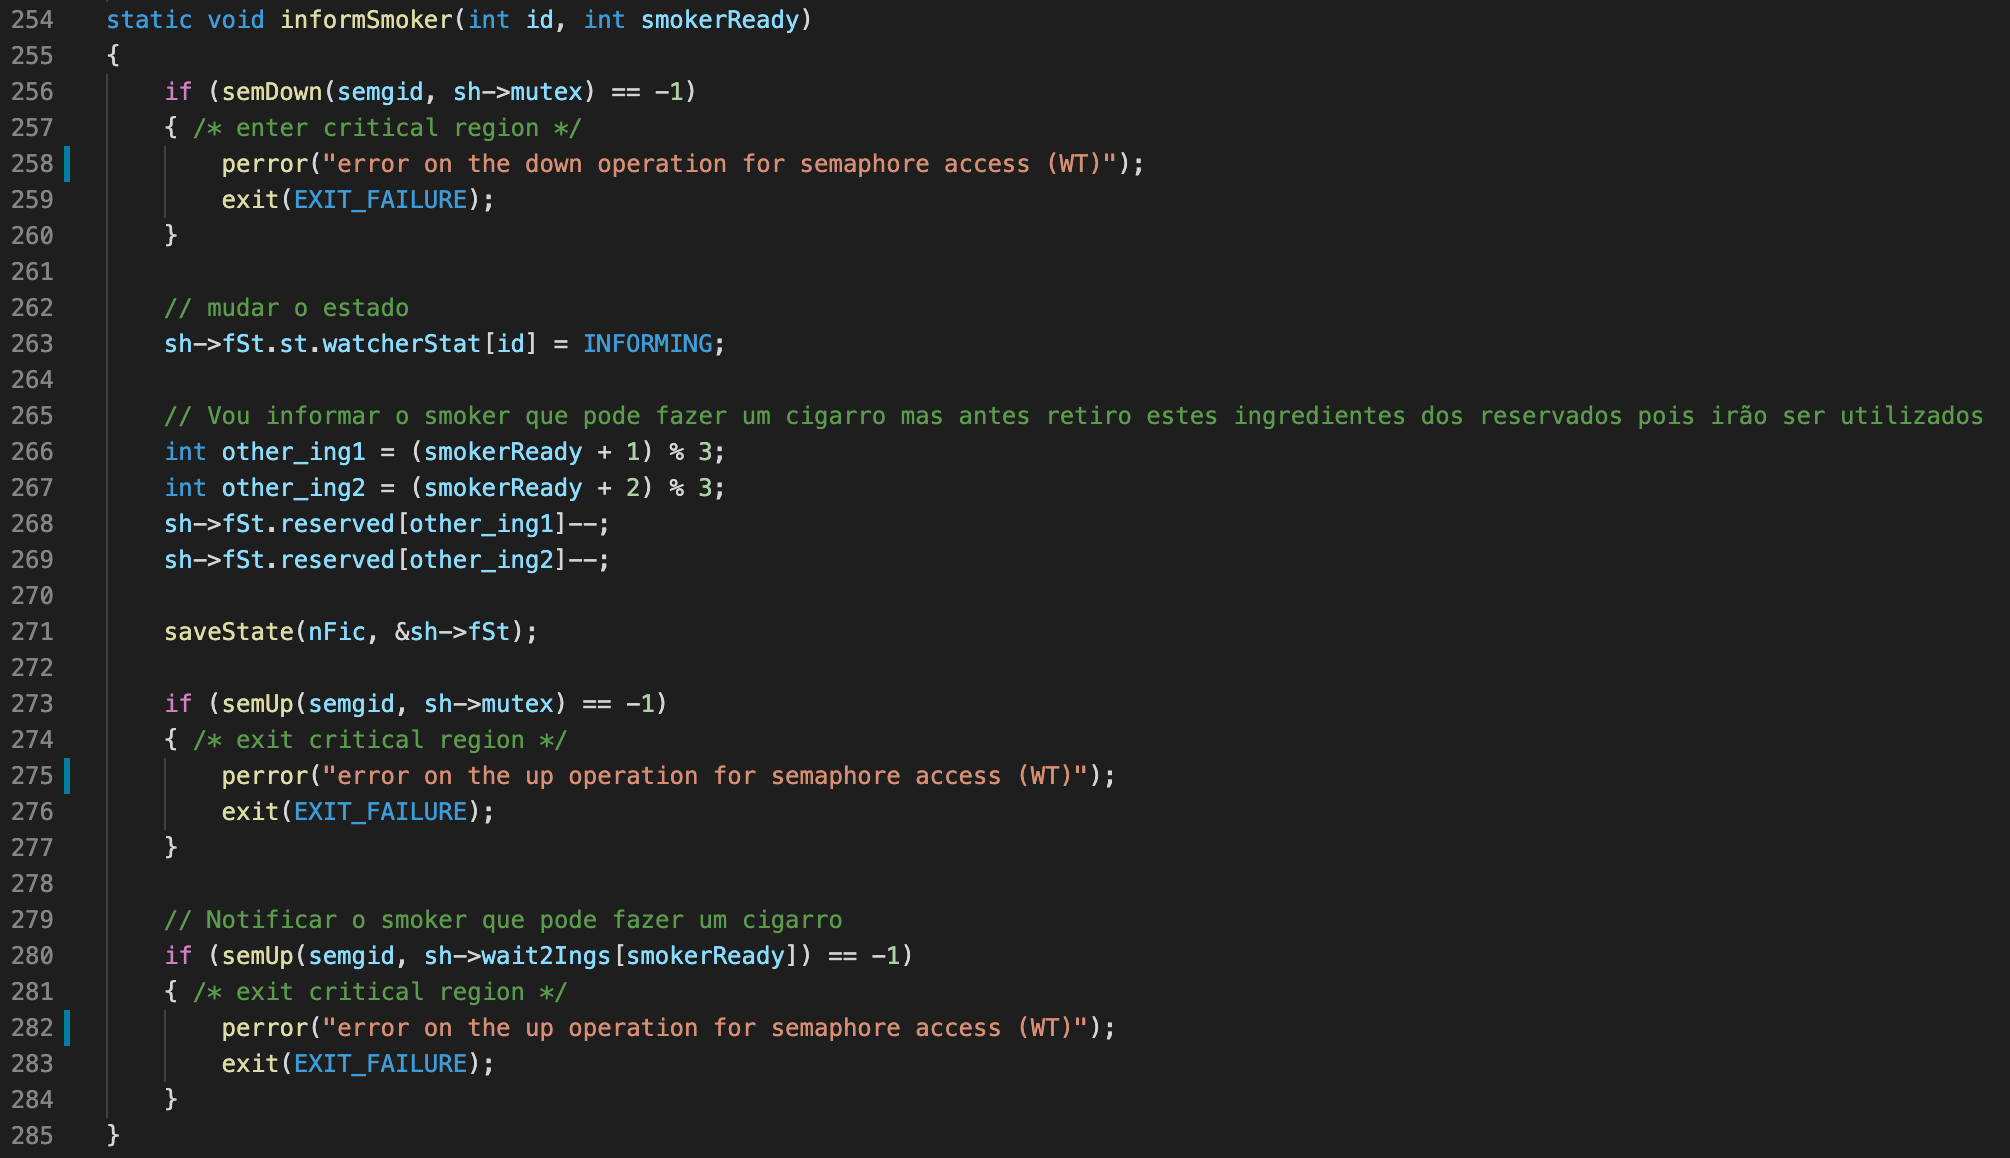
\includegraphics[width=\textwidth]{images/implementation/informsmok.png}
    \caption{Função \textit{informSmoker()}}
\end{figure}

\subsection{\textit{Smoker}}
\par Para implementar a solução da entidade \textit{Smoker} foi necessário alterar o ficheiro \textit{semSharedMemSmoker.c} nos locais assinalados. As funções \textit{waitForIngredients()}, \textit{rollingCigarette()} e \textit{smoke()} foram modificadas da maneira que se segue.

\subsubsection{\textit{waitForIngredients()}}

\par Na função \textit{waitForIngredients()} o Fumador espera pelos 2 ingredientes que ele não tem. Assim, dentro da região crítica, este atualiza o seu estado para \textit{WAITING\_2ING} e guarda em memória partilhada. Fora da região crítica, é bloqueado um semáforo, de modo ao Fumador esperar que o \textit{Watcher} o notifique da disponibilidade dos ingredientes. Posteriomente, volta-se a entrar na região crítica verificando-se se a flag \textit{closing} está a \textit{true}. Em caso afirmativo, é alterado o estado para \textit{CLOSING\_S} e o retorno da função para \textit{false}, guardando estes dados na memória partilhada. Em caso contrário, o Fumador vai retirar os ingredientes que irá usar do \textit{array} dos ingredientes.

\begin{figure}[!h]
    \centering
    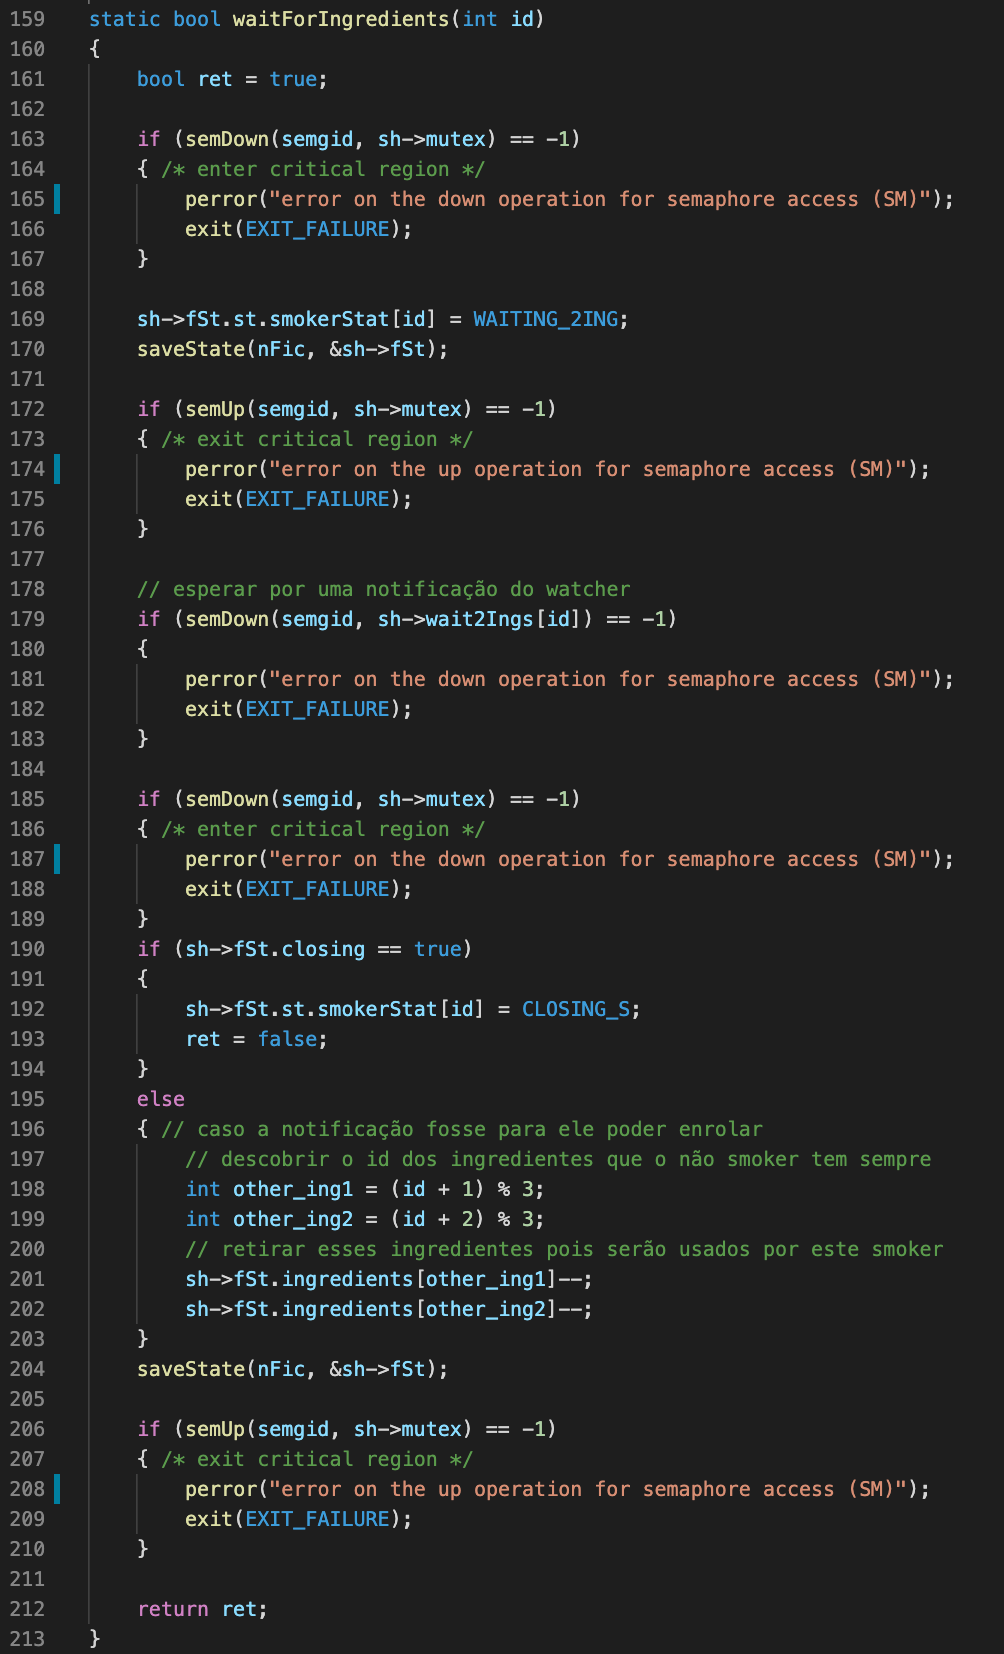
\includegraphics[scale=0.7]{images/implementation/waitforings.png}
    \caption{Função \textit{waitForIngredients()}}
\end{figure}

\clearpage

\subsubsection{\textit{rollingCigarette()}}

\par Ao executar \textit{rollingCigarette()} o Fumador vai enrolar um cigarro. Isto é alcançado entrando na região crítica, de modo a que o Fumador altere o seu estado para \textit{ROLLING}, guardando-o depois na memória partilhada. Fora da região crítica, se o tempo para enrolar o cigarro, gerado anteriormente, for maior que 0, o processo é suspenso durante esse tempo através da função \textit{usleep}. Antes da função terminar, é desbloqueado o semáforo \textit{waitCigarette} através do qual é notificado o \textit{Agent} que o Fumador acabou de enrolar.

\begin{figure}[!h]
    \centering
    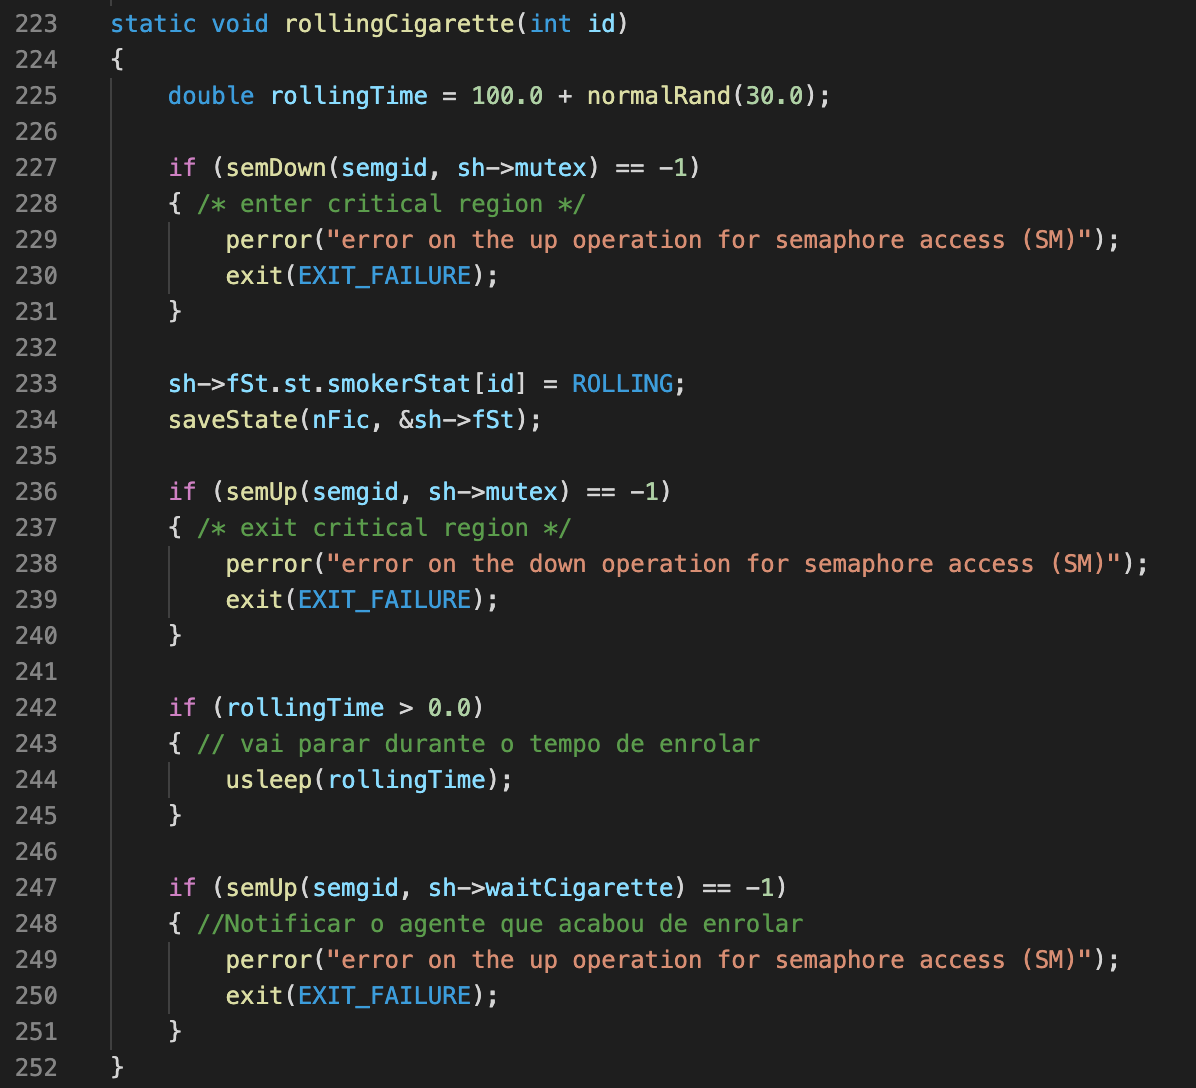
\includegraphics[width=\textwidth]{images/implementation/rolling.png}
    \caption{Função \textit{rollingCigarette()}}
\end{figure}

\clearpage

\subsubsection{\textit{smoke()}}

\par Na função \textit{smoke()} o Fumador vai fumar. Assim, na região crítica, é alterado o seu estado para \textit{SMOKING} e incrementado 1 à posição correspondente ao seu \textit{id} no \textit{array} dos cigarros fumados, guardando estes dados na memória partilhada. Já fora da região crítica, é gerado um tempo para fumar e se este for mais que 0, o processo é suspenso durante esse tempo através da função \textit{usleep}.

\begin{figure}[!h]
    \centering
    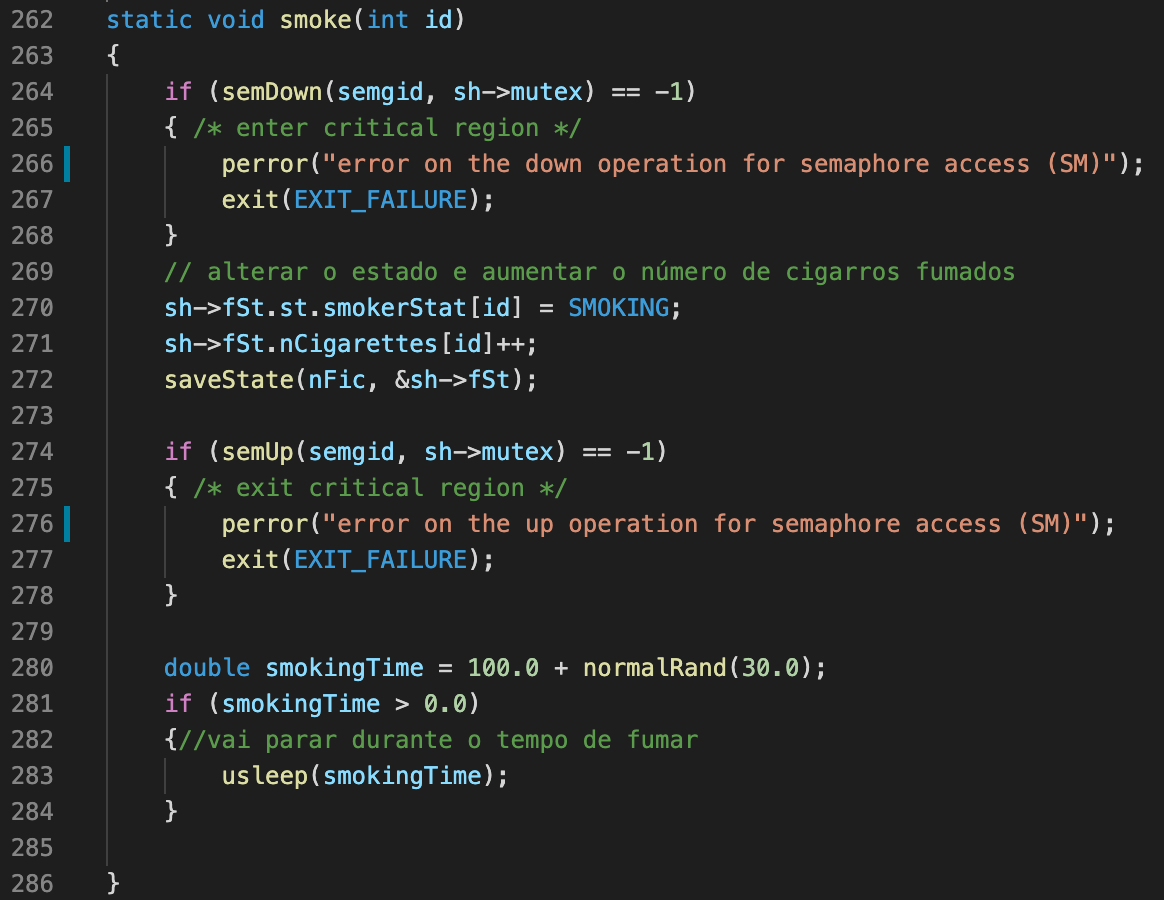
\includegraphics[width=\textwidth]{images/implementation/smoke.png}
    \caption{Função \textit{smoke()}}
\end{figure}



\clearpage

\section{Resultados}
\par Ao longo da criação de uma solução para este problema foram sendo realizados testes para confirmar que estávamos na direção certa. Teve-se sempre o cuidado de ir testando entidade a entidade, assim que se pensava ter a resolução correta, comparando o output com o do professor para verificar quaisquer discrepâncias que pudessem ser preocupantes e indicadoras de um erro.

\par Foram feitas 1000 execuções do programa, através do script \textit{run.sh} disponibilizado pelo professor, de modo a assegurar as condições referidas em cima. A imagem que se segue mostra o resultado da primeira execução, sendo que todas as execuções podem ser encontradas no ficheiro \textit{resultados.txt} na raiz da entrega.

\begin{figure}[!h]
    \centering
    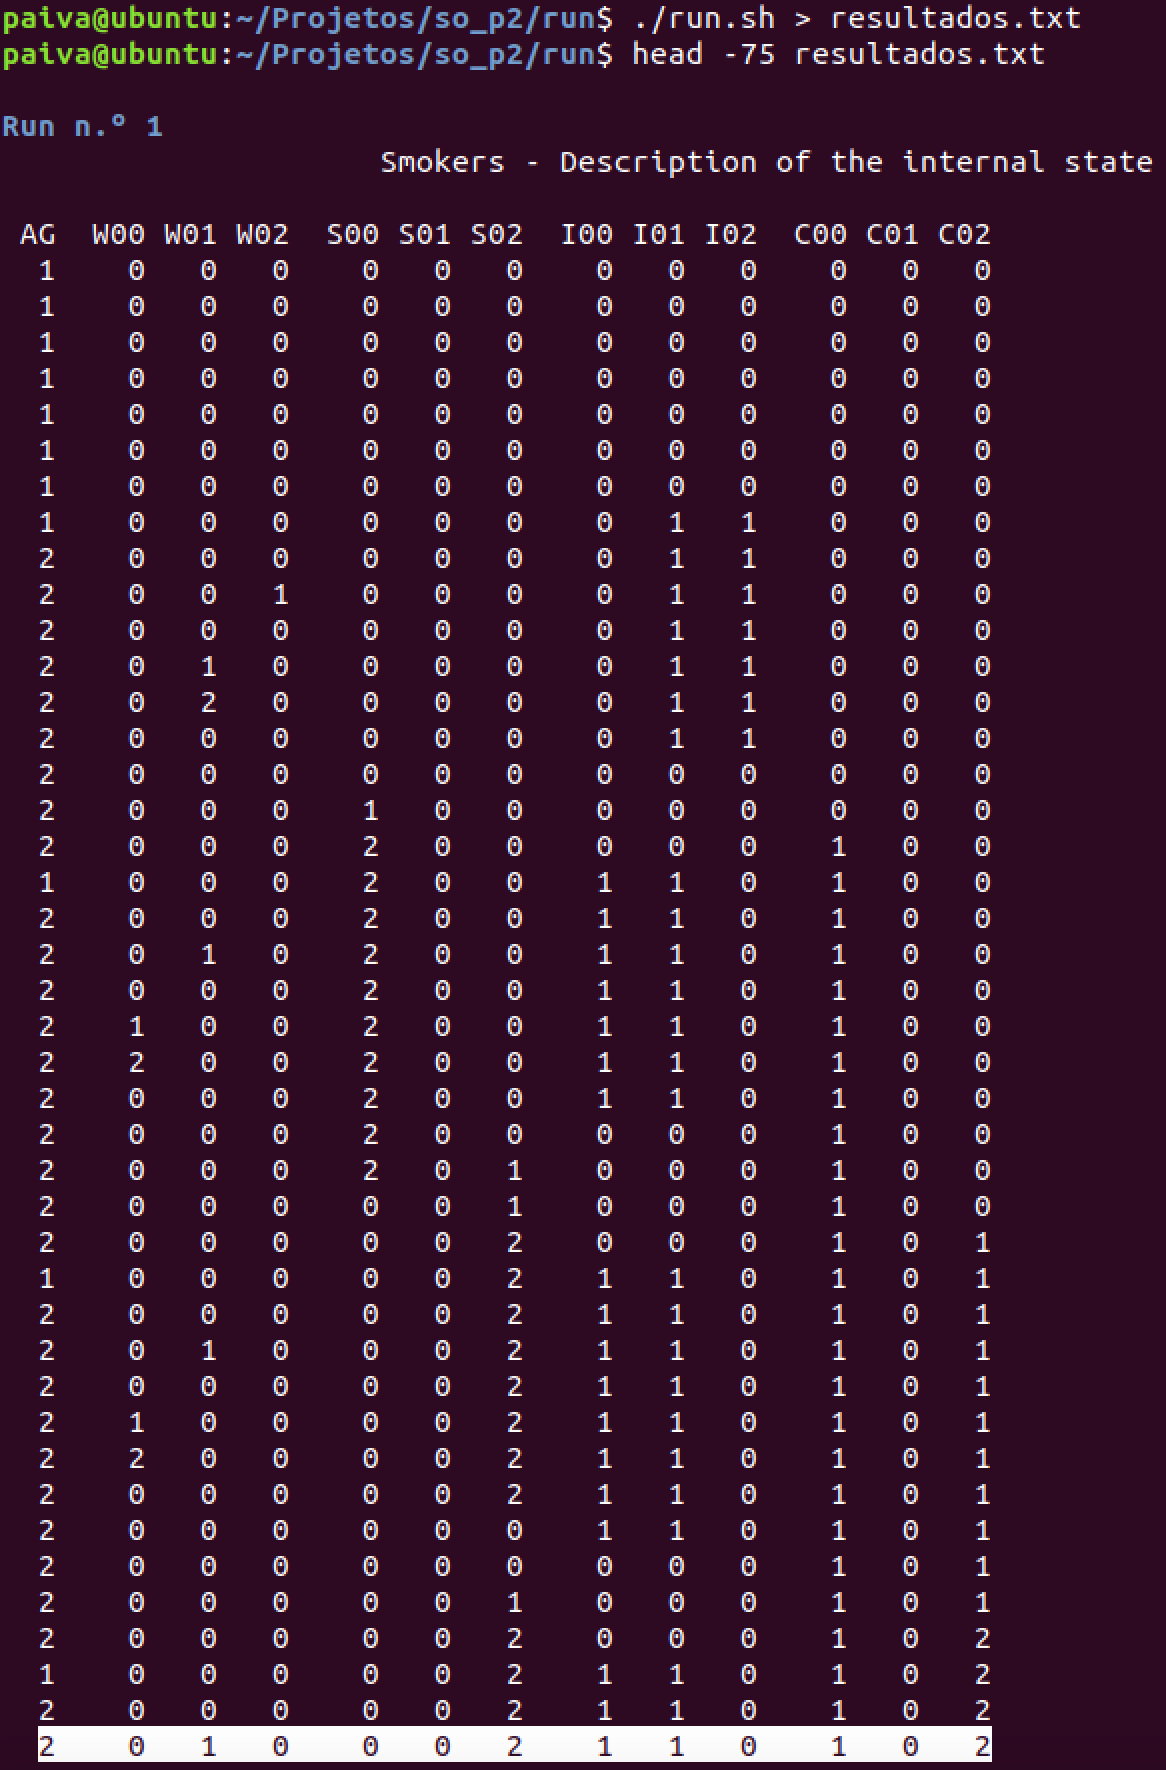
\includegraphics[scale=0.5]{images/resultados/res1.png}
\end{figure}
\clearpage
\begin{figure}[!tH]
    \centering
    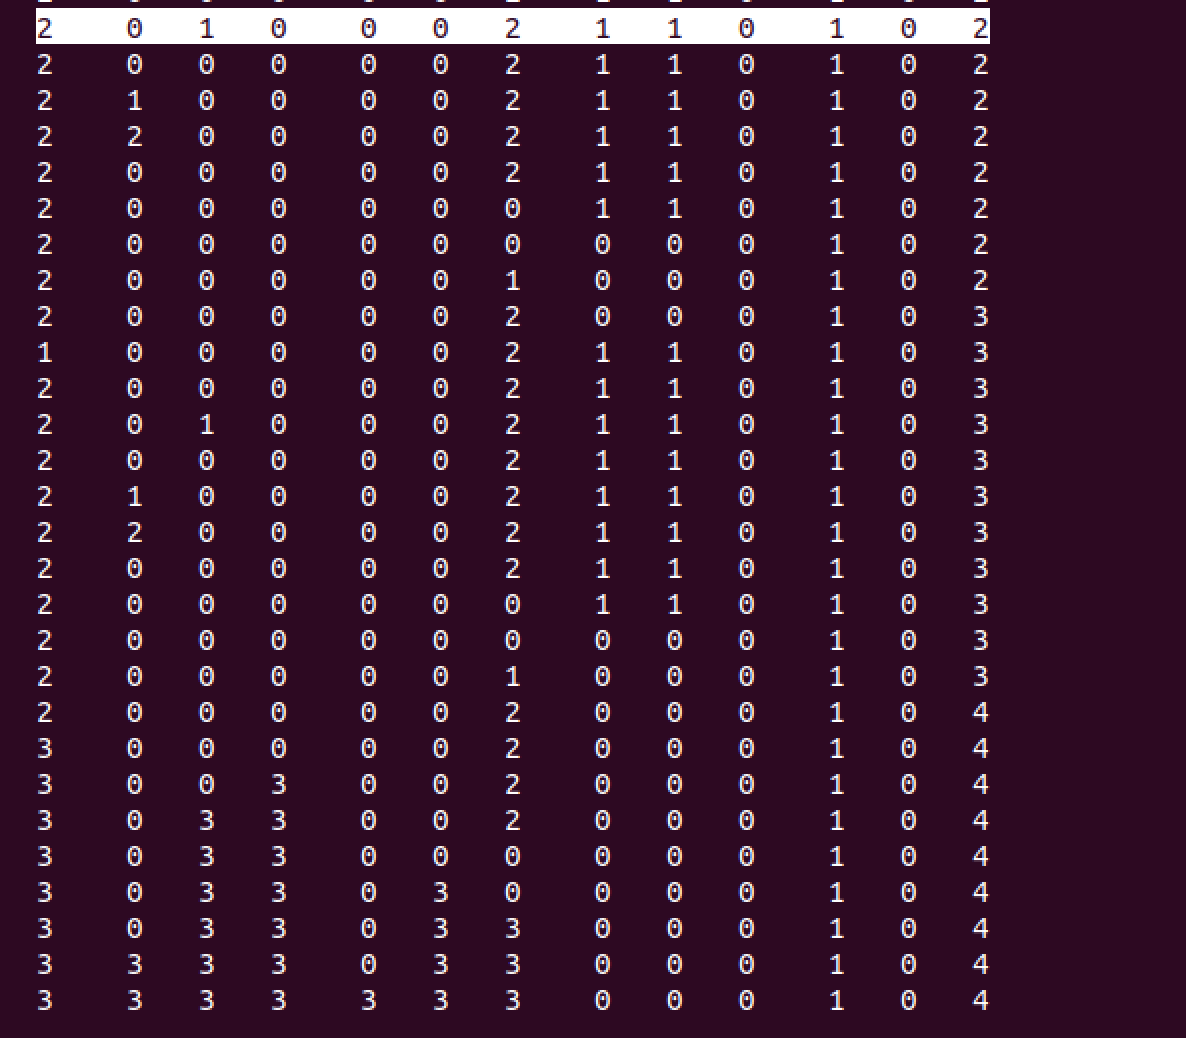
\includegraphics[scale=0.5]{images/resultados/res2.png}
    \caption{Resultados obtidos}
    \vspace*{10in} %forçar ir para cima
\end{figure}


\clearpage

\section{Conclusão}
\par Terminando, pensa-se que, de acordo com as metas estabelecidas pelo docente, o trabalho foi bem sucedido. Uma das principais dificuldades sentidas esteve relacionada com a primeira análise e compreensão de todo o código previamente escrito pelo professor. No entanto, assim que se finalizou uma das entidades, percebendo-se bem a sua implementação, facilmente se desenvolveu o resto do trabalho.
\par Aprofundaram-se os conhecimentos sobre o funcionamento de semáforos e sincronização de \textit{threads}, sendo mais simples interiorizar certos pormenores a partir de um projeto como este, da mesma maneira que através da realização dos guiões práticos propostos sobre estes temas.
\par Assim sendo, como os resultados obtidos podem ser considerados semelhantes aos do docente, é concluído que esta poderá ser uma das possíveis soluções.

\clearpage

\section{Bibliografia}

\bibliographystyle{plain}

\bibliography{biblist}

\vspace{5mm} %5mm vertical space

[1] \url{http://index-of.es/Java/Operating%20System%20Concepts%20with%20Java%208th.pdf}


\end{document}

